% 英文で執筆する場合はクラスファイルへのオプションを[T,E]としてください.
% If you want to write your paper in English, pass to [T,E] options to document class.
\documentclass[T,J]{fose} % 「コンピュータソフトウェア」用のクラスファイルは compsoft です.
\taikai{2023} % 固定です.出版委員長が毎年変更してAuthor Kitを配布してください.

\usepackage [dvipdfmx] {graphicx}
\usepackage{multirow}
\usepackage{caption}

% ユーザが定義したマクロなどはここに置く.ただし学会誌のスタイルの d
% 再定義は原則として避けること.

% 以下は説明のために使用したパッケージであるため,削除可能.
\usepackage{fancyvrb}
\usepackage{xurl}
\usepackage{cite}
\usepackage{color}
\usepackage{graphicx}
\usepackage{ascmac}
% \usepackage[dvipdfmx]{color} クラッシュしていてなくても動くのでコメントアウト


\newcommand{\todo}[1]{\colorbox{yellow}{{\bf TODO}:}{\color{red} {\textbf{[#1]}}}}
\newcommand{\done}[1]{\colorbox{green}{{\bf DONE}:} {\textbf{[#1]}}}


\begin{document}

% 論文のタイトル
\title{Scratchにおけるプログラム類似度とオブジェクト\\動作軌跡類似度の分析}
% 以下の \etitle(と\@etitle)はFOSE論文フォーマット独自のマクロです.
% FOSEに投稿した論文を発展させてコンピュータソフトウェアに投稿される場合はコメントアウトしてください.
% \setetitleは奇数ページのヘッダに表示する文字列(\etitle)を設定するためのマクロです.
% タイトルが2行に渡る場合は "\\" を 使用することで任意の位置で改行をすることができます.
\setetitle{An Analysis of Program Similarity and Object Motion Trajectory Similarity between Scratch Works}
%\setetitle{Long Long Long Long Long Long \\ Long Long Long Long Long \\ Long Long Long Long Long Long Long Long Long Long Long Long Paper Title}

% タイトル,著者などが複数行にわたり,論文冒頭の著者名が日本語アブストと重複して描画された場合に以下のコメントアウトを外してください.
%\longtitle

% 著者
% 和文論文の場合,姓と名の間には半角スペースを入れ,
% 複数の著者の間は全角スペースで区切る
%
\author{岡本 圭悟 伊原 彰紀
%
% ここにタイトル英訳 (英文の場合は和訳) を書く.
% 英語タイトルは論文1ページ目左下,著者らの名前・所属一覧の一番上に表示される
%
% 上記\setetitle中で改行した場合は "\etitle" を削除し,改行(\\)を入れていないタイトルを記載してください.
% \ejtitleは1ページ目左下に挿入されるタイトルとして使用されます.
% また,"\etitle"はFOSE論文フォーマット独自のマクロです.
%\ejtitle{\etitle}
%
% ここに著者英文表記 および
% 所属 (和文および英文) を書く.
% 複数著者の所属はまとめてよい.
%
% 複数著者の所属は以下のようにまとめてよい.
\shozoku{Keigo Okamoto, Akinori Ihara}{和歌山大学システム工学部}
{Faculty of Sytstems Engineering, Wakayama University}
}

%
% 和文アブストラクト
% In English paper, content of Jabstract will be ignored. 
\Jabstract{
ビジュアルプログラミング言語Scratchでは,ユーザが制作した作品をオンライン上に公開することができ,またユーザは公開された作品の中から実現したい動作を検索することで,実装の参考にすることができる.ただし,検索結果にはプログラムは類似するが,学習者が実現したい振る舞いを持たない作品も多く含まれる.このように実行結果の類似性とプログラムの類似性の乖離は,プログラミング検索における多様な実装方法を持つ作品の収集を妨げ,学習効率の低下につながると示唆する.本研究では,Scratchにおけるプログラムが類似する作品の違いを分析するために,Scratchにおいて制作されるプログラムの類似度の測定手法,およびオブジェクト動作軌跡の類似度の測定手法を提案する.また,ケーススタディとして4000件のScratch作品を対象に,プログラムが類似するか否か,オブジェクト動作軌跡が類似するか否かの4種類に分類し,作品群毎に特徴を分析する.
}
%
% 英文アブストラクト(本サンプルの原論文にはなし)
%\Eabstract{
%\todo{英文アブスト}
%}
%
\maketitle \thispagestyle {empty}
%%%%%%%%%%%%%%%%%%%%%%
\section{はじめに}
%%%%%%%%%%%%%%%%%%%%%%
我が国でも,プログラミング的思考力の育成を目的とし,プログラミング教育を本格的に推進している.特に,ビジュアルプログラミングは,画像オブジェクトの移動,効果音の制御などを命令処理を持つブロックを組み合わせることで直観的にプログラムの実装をおこなうことができる開発環境として,プログラミング初学者に広く利用されている.プログラミング的思考力の育成に,ビジュアルプログラミング言語を用いた教育が有効であることが明らかにされている\cite{}\cite{}.ビジュアルプログラミングのオンライン開発環境であるScratchは世界中の教育機関やプログラミング教室で利用されている.
%杉浦学,松澤芳昭,岡田健,大岩元.アルゴリズム構築能力育成の導入教育:実作業による概念理解に基づくアルゴリズム構築体験とその効果.情報処理学会論文誌,Vol.49,No.10,pp.3409-3427,2008.
%森秀樹, 杉澤学, 張海, 前迫孝憲.Scratchを用いた小学校プログラミング授業の実践 : 小学生を対象としたプログラミング教育の再考(教育実践研究論文).日本教育工学論文誌,Vol.34, No.4, pp.387–394, 2011.

Scratchでは,ユーザが制作したプログラム作品にタイトルや作品の説明文を付けてオンラインサービス上に公開することができ,2023年7月時点には1億3500万件\footnote{Scratch Statistics: \url{https://scratch.mit.edu/statistics/}}を超える作品が公開している.Scratchは公開済みの作品を対象に自然言語による作品検索サービスを提供しており,公開済み作品の中からユーザが制作したい作品,実現したい動作を検索し,実装の参考にする\cite{}.
%Mitchel Resnick, John Maloney, Andr´es Monroy-Hern´andez, Natalie Rusk, Evelyn Eastmond, Karen Brennan, Amon Millner, Eric Rosenbaum, Jay Saul Silver, Brian S Silverman, Yasmin Bettina Kafai, Scratch: Programming for all, Communications of the ACM, Vol.52, No.11, pp.60-67, 2009.
Scratchで制作する作品は小規模なプログラムが多く,使用するブロックも限られているため,検索によって類似するプログラムを含む作品が多数出力される.その一方で,検索結果にはプログラムは類似するが,XXXのため学習者が実現したい振る舞いを持たない作品も多く含むことが示唆される.
% \todo{ここはもう少し書きたい}
実行結果の類似性とプログラムの類似性の乖離は,プログラミング検索における多様な実装方法を持つ作品の収集を妨げ,学習効率の低下につながると示唆する.

本研究は,Scratchにおけるプログラムが類似する作品とオブジェクト動作軌跡が類似する作品の違いを分析するために,Scratchにおいて制作されるプログラム類似度の計測方法,およびオブジェクト動作軌跡の類似度の計測方法を提案する.プログラム類似度の計測方法にはプログラムの編集距離を用いる(3章).オブジェクト動作軌跡類似度の計測方法には動的時間伸縮法(DTW: Dynamic time warping)を用いる(3章).本研究では,ケーススタディとしてScratchAPIを用いてランダムに収集し,条件に基づいてフィルタリングした4000件の作品を対象に,プログラムが類似するか否か,オブジェクト動作軌跡が類似するか否かの4種類に分類し,それぞれの作品の特徴を分析する.

続く\ref{sec:RelatedWork}章は本論文の立ち位置を説明するための関連研究と研究動機を述べる.\ref{sec:Similarity measurement}章は本論文で用いる類似度の測定手法を述べ,\ref{subsec:Analyze related work}章はケーススタディで用いるデータセットとアプローチ,その結果と考察を述べる.

%%%%%%%%%%%%%%%%%%%%%%
\section{Scratchにおける作品間の類似度}\label{sec:RelatedWork}
%%%%%%%%%%%%%%%%%%%%%%

\subsection{ビジュアルプログラミング言語Scratch}\label{subsec:Scratch}

ScratchはMITメディアラボが開発するビジュアルプログラミング言語の開発環境であり,利用者はプログラムの命令処理を持つブロックを組み合わせることプログラミングを行うことができる.特に,画像オブジェクトの移動,効果音の入出力などをプログラムで制御することによりゲームやアニメーションなどの作品が多数制作される.図\ref{fig:Scratch-description}にScratch3.0における作品制作画面を示す.Scratchにおける作品は主にブロック,スクリプト,スプライトの3つの要素で構成される.
\begin{itemize}
\item ブロック:プログラムを構成する最小の単位であり,それぞれ特定の命令処理を持つ.ユーザは図\ref{fig:Scratch-description}の(1)に示したようなブロックを組み合わせることでプログラムを実装する.Scratchでは,画像の移動を制御する座標移動ブロック,条件分岐や繰り返しなどの制御ブロックなどが提供されており,種類に応じて役割,色,形が異なる.
\item スクリプト:図\ref{fig:Scratch-description}の(2)に示すように複数のブロックを組み合わせて一つにしたプログラムを指す.特に,スクリプトの先頭にはプログラムを開始するイベントブロックを使用し,スクリプトを開始するためのトリガーが設定する.同じイベントブロックを持つスクリプトが並列に存在する場合は,同時にスクリプトを実行開始することができる.
\item スプライト:図\ref{fig:Scratch-description}の(3)に示すように作品中に使用する画像オブジェクトを指す.各スプライトには,一つ以上のスクリプトが紐づいており,スプライトは実行画面上で,スクリプトに含まれる命令処理の通りに動作する.
\end{itemize}
\begin{figure}[t]
	\centering
	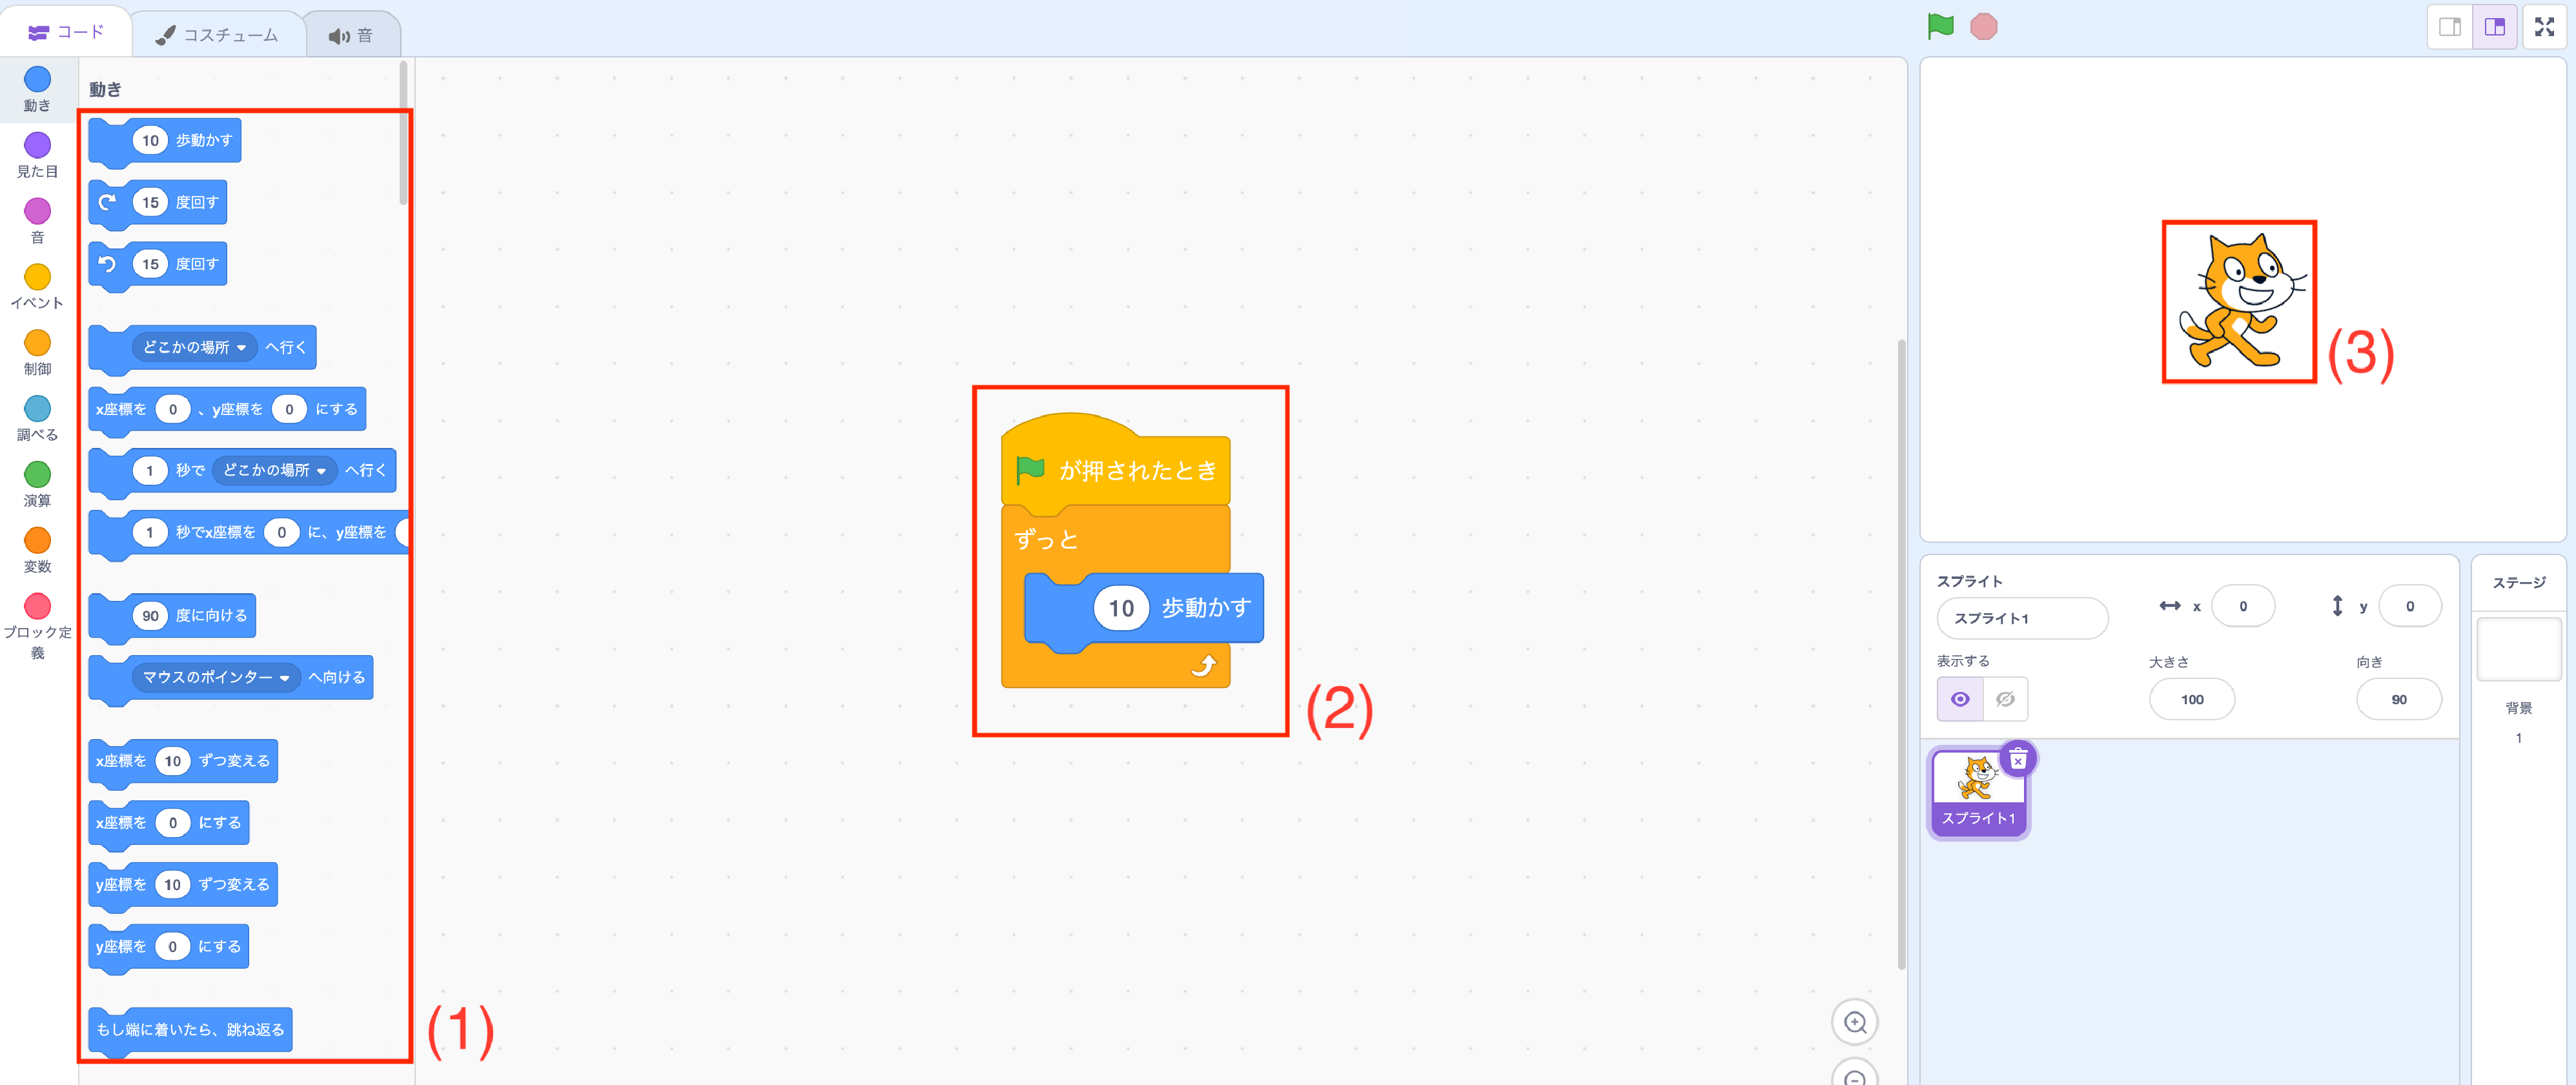
\includegraphics[width=1.0\linewidth]{Okamoto_fig/Scratch-description.pdf}
	\caption{Scratchの作品制作画面}
	\label{fig:Scratch-description}
\end{figure}
%\subsection{従来研究:動作軌跡の類似度}
%Scratchで,ユーザはキーワード検索によって他者の作品を参照することができるが,ユーザが思い描く動作軌跡を言語化して検索することは容易でない.従来研究では,マウスを用いた描画によってユーザの動作イメージを入力することで,動作の言語化を必要としないScratch作品の直観的作品検索手法を提案している.入力と検索対象となるスプライトの動作軌跡の類似度合いを測定するために,2つの時系列データの距離を算出する動的時間伸縮法(以下,DTW)を用いており,類似動作を抽出可能な距離を明らかにした.

\subsection{従来研究: Scratchにおけるプログラム解析}\label{subsec:analyze-scratch}

Scratchをはじめとするビジュアルプログラミング言語を用いて開発されるプログラムの調査をおこなう研究が多数報告されている.
%Re-Use of Programming Patterns or Problem Solving?Representation of Scratch Programs by TGraphsto supportStatic Code Analysis@WiPSCE2020
Peeratham\cite{Understanding}らは,ビジュアルプログラミングの作品に含まれるコードスメルを調査しており,プログラムで頻繁に発生する品質問題を特定し,作品を分類している.
%Understanding Recurring Quality Problems and Their Impact on Code Sharing in Block-Based Software@VLHCC2017
また,Peeratham\cite{techapalokul2019code}らは,ビジュアルプログラミングにおけるリファクタリングツールの適用による効果を調査しており,再利用されるプログラムを分類している.
%Code Quality Improvement for All: Automated Refactoring for Scratch@VLHCC2019
%Behavior-based clustering of visual code @VLHCC2015
従来研究では,総じてプログラムの分類には取り組んでいるが,個々のプログラムの類似性には着目されておらず,またプログラムによって移動する画像オブジェクトの動作軌跡の類似性も確認していない.
% \todo{なぜ確認しないといけないのか?}

\subsection{従来研究:プログラムの類似度}\label{subsec:similarity of scratch}
テキストベースのプログラミング言語であるC言語やJava言語を対象としたプログラム検索手法として,特徴ベクトルに基づく手法,機械学習に基づく手法,データベースに基づく手法など,プログラムの類似性に着目する研究が多数報告されている\cite{}.
%Luca Di Grazia and Michael Pradel. 2023. Code Search: A Survey of Techniques for Finding Code. ACM Comput. Surv. 55, 11, Article 220 (November 2023), 31 pages. https://doi.org/10.1145/3565971

テキストベースのプログラミング言語に対して,ビジュアルプログラミング言語であるScratchでは,プログラムの実行結果が視覚的に出力されるため,プログラムの実装方法が類似していても,スプライトの動作軌跡は類似しないことが多々ある.このことから,Scratch上ではプログラムが類似していても,一概に似ている作品であるとは言えず,プログラムの出力結果であるスプライトの動作軌跡も考慮する必要がある.

%Scratchで,ユーザは類似するプログラムが混在する膨大な検索結果の中から,多様なプログラムの実装方法を含む作品を探すことは手間がかかり容易でない.従来研究では,Scratch作品において類似したプログラムの実装方法を持つ作品を各々紐づけるために,類似プログラムを判定するための手法を提案した.具体的には,Scratchプログラムを抽象構文木(以下,AST)として捉え,プログラム間の編集距離をプログラムの類似度として算出しており,類似プログラムを判定するための基準を明らかにした.



\subsection{動機}\label{subsec:reason}

本研究では,図\ref{fig:sample-scatter}に示すように,プログラムが類似するか否か,オブジェクト動作軌跡が類似するか否かの4種類に分類する.特に,図中の(2)に示すような第2象限(プログラムは類似するが,オブジェクト動作軌跡が類似していない),図中の(4)に示すような第4象限(オブジェクト動作軌跡は類似するが,プログラムは類似していない)のような,プログラムの類似度とオブジェクト動作軌跡類似度が乖離する作品を分析する.

第2象限の事例を図\ref{fig:pattern1}に示す.図\ref{fig:pattern1}中の(1),(2)のプログラムはそれぞれ類似していると言えるが,(1)の作品のオブジェクトは四角の形を描き,(2)の作品のオブジェクトは円の形を描くため,動作軌跡は類似していないといえる.これは,角度を変えるブロックの数値の差がオブジェクトの動作軌跡に影響したことが原因である.このように,ブロック内の数値が異なると,プログラムが類似しても動作軌跡が類似しないことが示唆される.

第4象限の事例を図\ref{fig:pattern2-1}と図\ref{fig:pattern2-2}に示す.図\ref{fig:pattern2-1}は(1)も(2)もオブジェクトが右に移動する同じ動作軌跡を描くプログラムだが,プログラム自体は類似していないことがわかる.Scratchでは座標の移動に関わるブロック以外にも,(2)内で示されているような見た目を変更するブロックや音を鳴らすブロックが提供されている.そのため,座標ブロック以外のブロックが作品内に多く存在すると,動作軌跡が類似してもプログラムが類似しないことが示唆される.

また,図\ref{fig:pattern2-2}も2つとも同じ動作軌跡を描くプログラムであるが,プログラムが類似していない作品である.この作品では,座標ブロック以外のブロックはあまり多く存在しないが,(1)ではループを用いて実装,(2)ではループを用いずに,そのままブロックを連ねて実装といったように,実装方法の違いでプログラムが類似しないことが示唆される.

\begin{figure}[t]
	\centering
	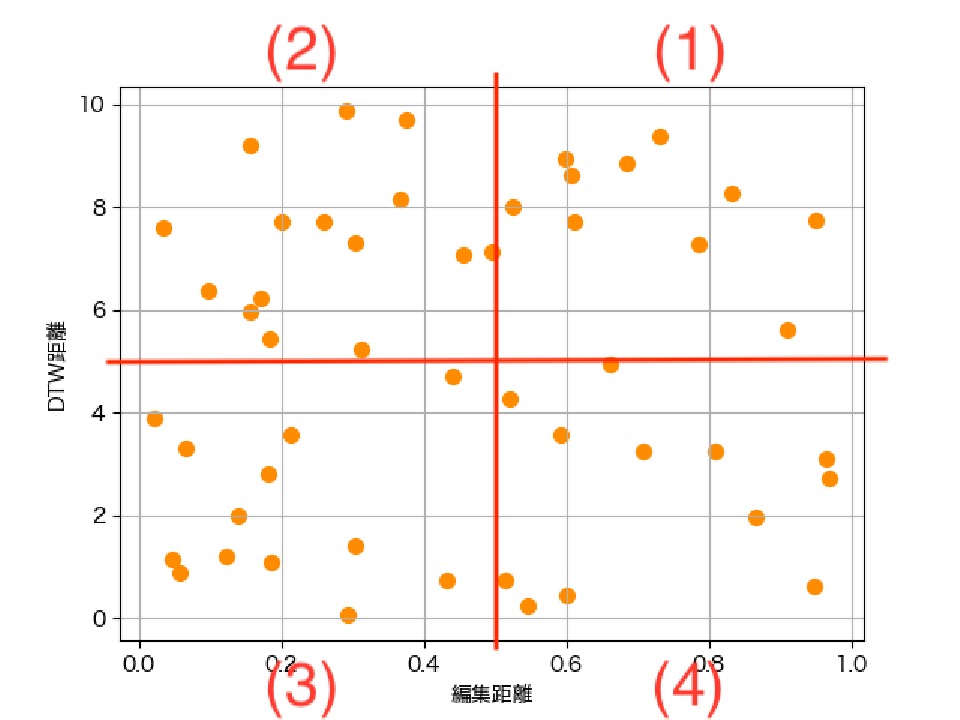
\includegraphics[width=1.0\linewidth]{Okamoto_fig/out-sample.pdf}
	\caption{編集距離とDTW距離の関係性を示した散布図の例}
	\label{fig:sample-scatter}
\end{figure}

\begin{figure}[t]
	\centering
	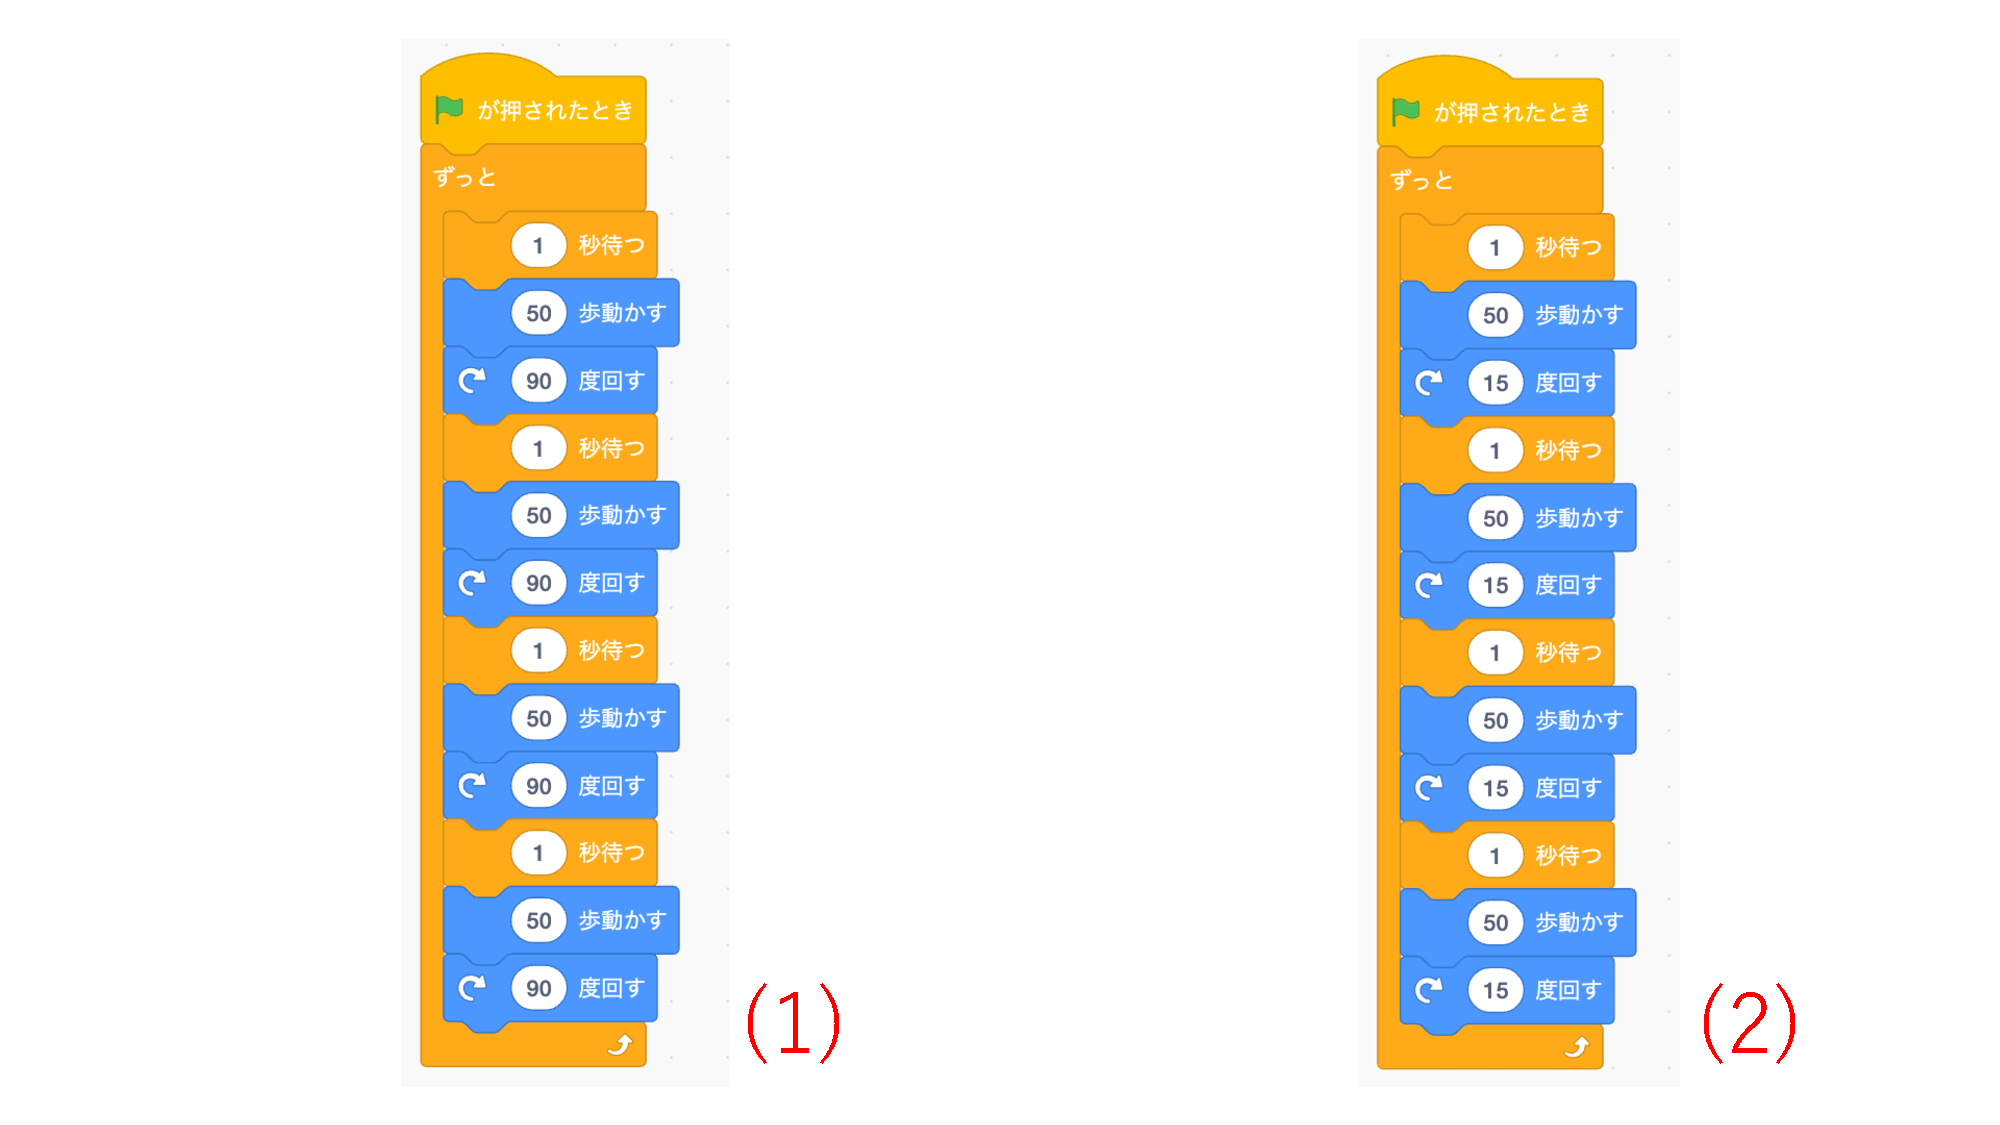
\includegraphics[width=1.0\linewidth]{Okamoto_fig/pattern1.pdf}
	\caption{プログラムは類似するが,オブジェクト動作軌跡が類似していない作品の例}
	\label{fig:pattern1}
\end{figure}
\begin{figure}[t]
	\centering
	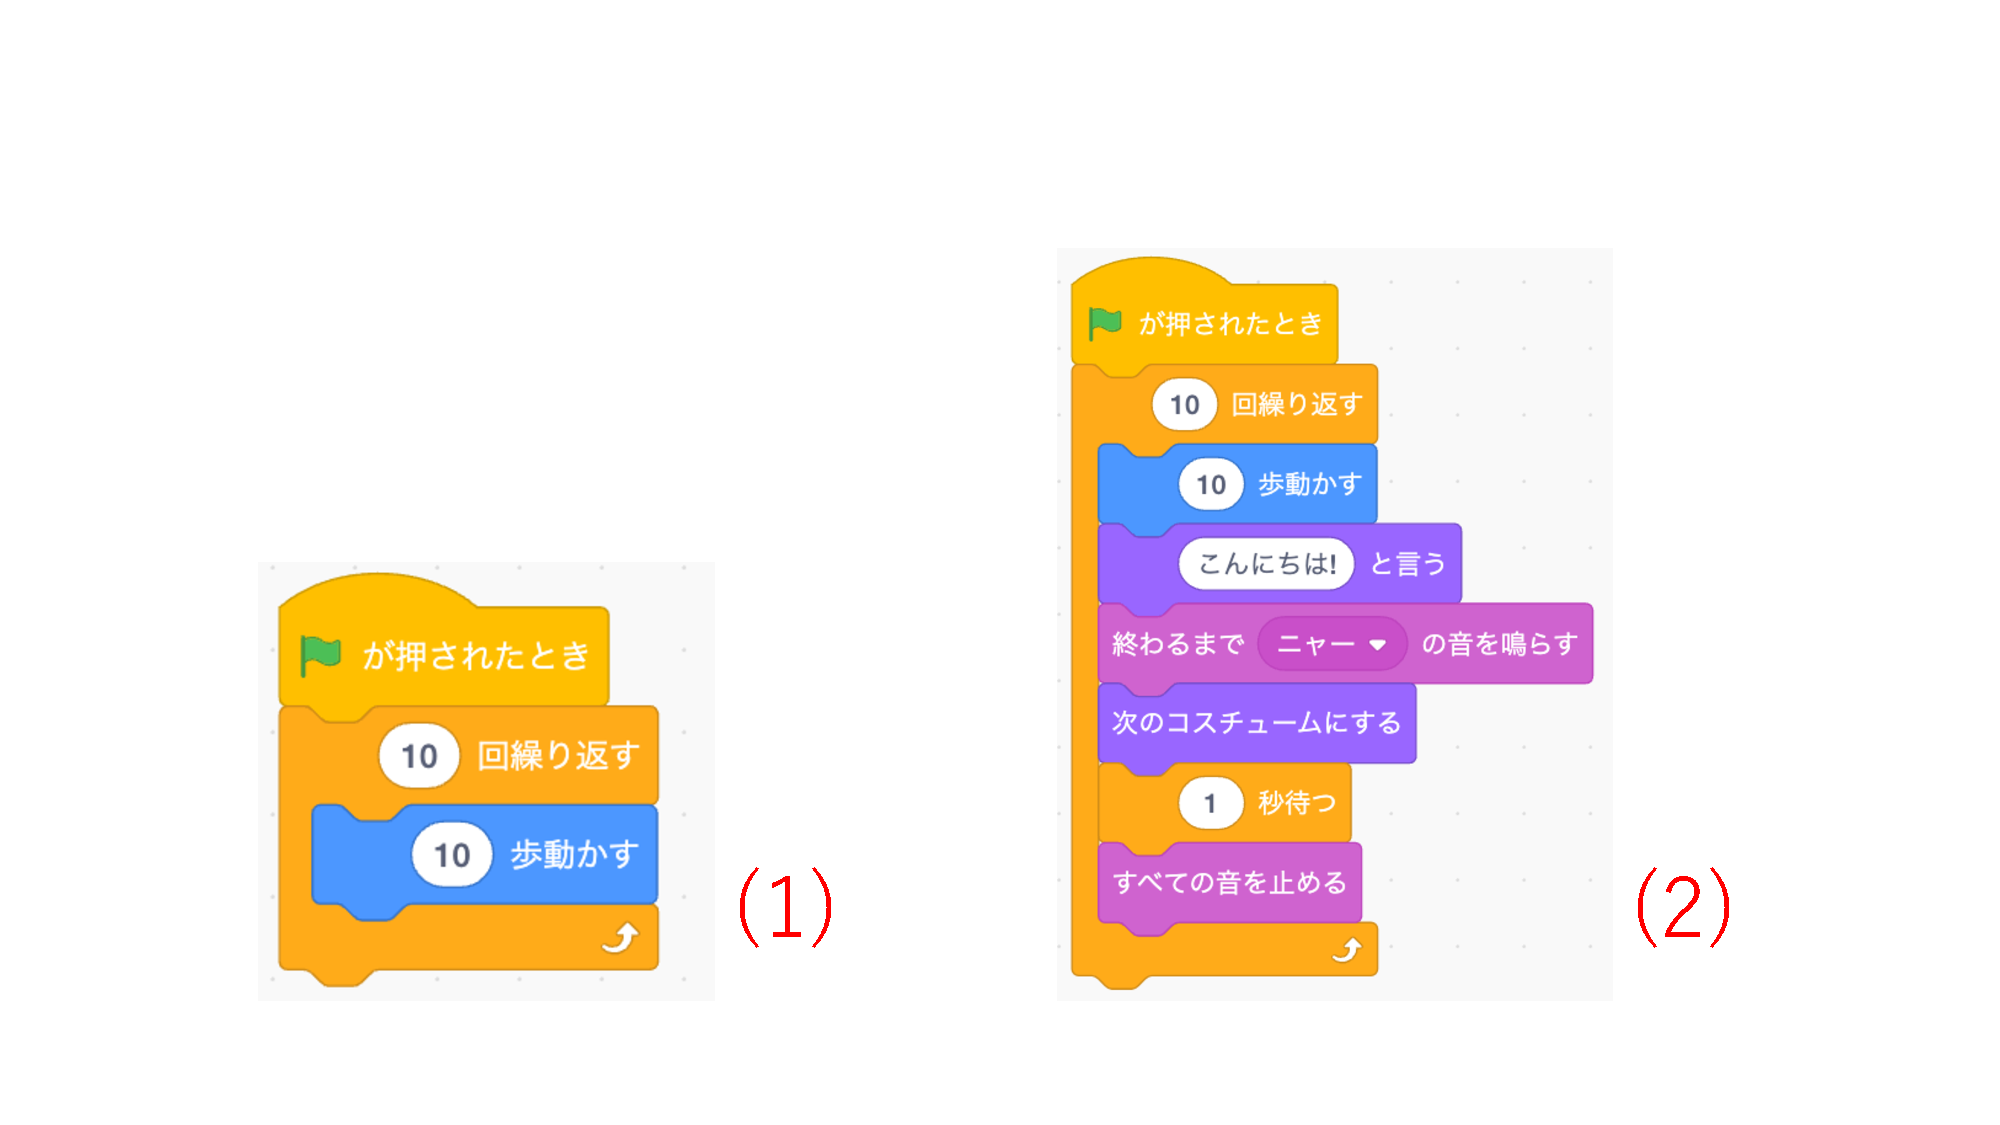
\includegraphics[width=1.0\linewidth]{Okamoto_fig/pattern2-1.pdf}
	\caption{オブジェクト動作軌跡は類似するが,プログラムが類似していない作品の例1}
	\label{fig:pattern2-1}
\end{figure}

\begin{figure}[t]
	\centering
	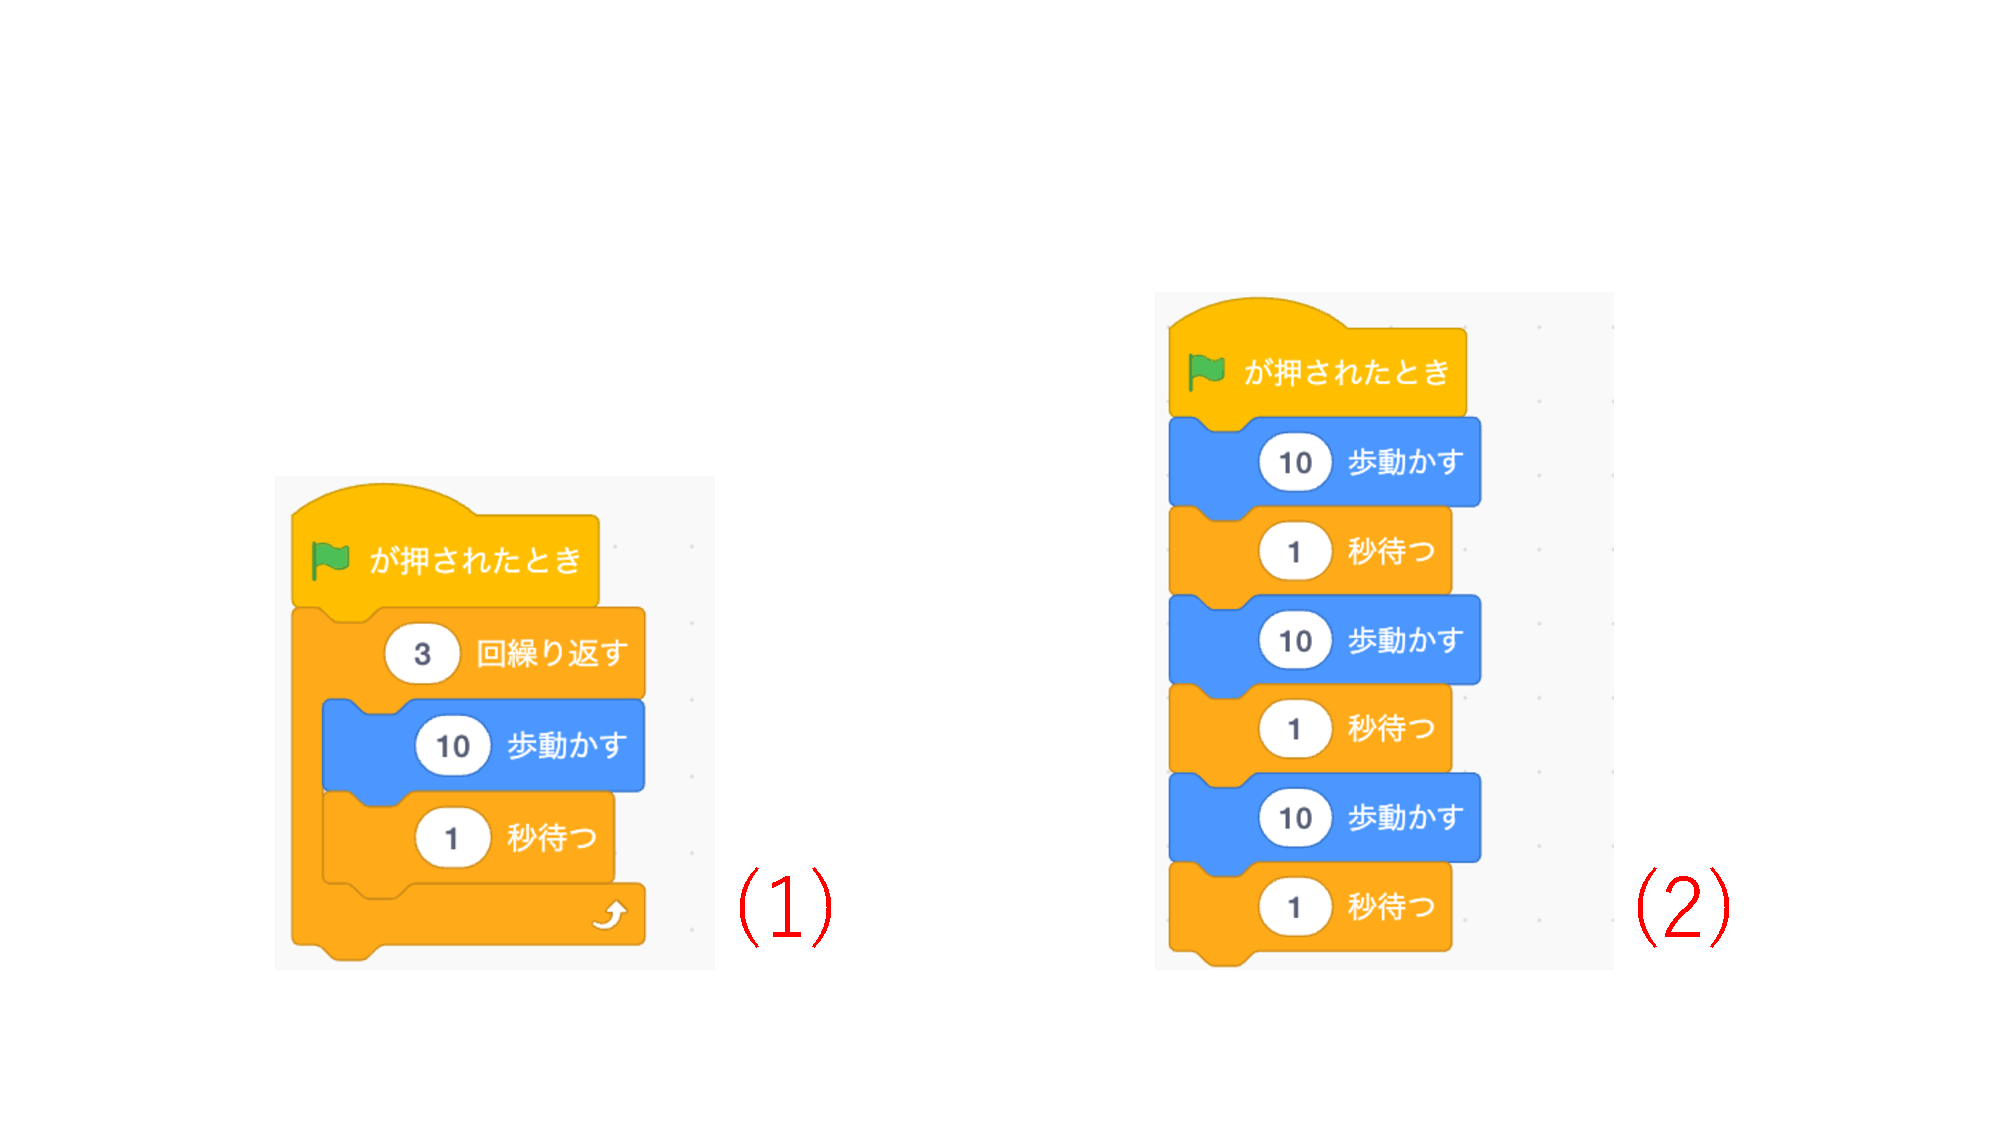
\includegraphics[width=1.0\linewidth]{Okamoto_fig/pattern2-2.pdf}
	\caption{オブジェクト動作軌跡は類似するが,プログラムが類似していない作品の例2}
	\label{fig:pattern2-2}
\end{figure}


\begin{itembox}[l]{Research Question}
同作品間における動作軌跡の類似度とプログラムの類似度に相関はあるか
\end{itembox}

%%%%%%%%%%%%%%%%%%%%%%
\section{類似度の測定手法}\label{sec:Similarity measurement}
%%%%%%%%%%%%%%%%%%%%%%

本章では,スプライトの動作軌跡の類似度,およびプログラムの類似度の算出方法について述べる.

\subsection{動作軌跡の類似度測定手法}\label{subsec:Similarity movement measurement}

作品に含まれるスプライトの移動軌跡の類似度を算出するために,本研究ではスプライトの座標の移動軌跡を追跡し,異なる作品に含まれるそれぞれのスプライトの移動軌跡の類似度を算出する.著者らは,先行研究\cite{}において動作軌跡の類似度を測定手法を開発しており,2つの手順(1. スプライトを配置する座標の時系列データの取得,2. 2作品間のスプライトの移動軌跡の類似度を算出)により類似度を算出する.

\subsubsection{スプライトを配置する座標の時系列データの取得}

先行研究\cite{}では,異なる作品に含まれるスプライトの移動軌跡を追跡するために,Scratchの作品中の実行画面内でスプライト画像の移動をLoweが提案したSIFT(Scale-Invariant Feature Transform)を用いて画像中の特徴点を抽出し,スプライトの座標変化を取得していた.しかし,当該手法は事前に追跡対象とするスプライト画像を決定するため,Scratchが提供する画像のみが対象となり,分析対象とする作品数が限られてしまう.また,実行画面の動画を事前に取得する必要があり,データ収集に膨大な時間を要することが課題であった.これらの課題解決として,本研究ではScratch APIにより取得できる作品で使用されるブロック情報に基づき,次の手順でスプライトの座標を追跡する.
\begin{enumerate}
    \item Scratchが公開しているAPIを用いて作品情報を含むJSONファイルを取得し,複数スプライトがある場合は先頭に存在するスプライトのスクリプト,ブロック情報を抽出
    \item ブロックを実行順序順にソートして,座標変化を含むブロックから座標情報を抽出
    \item 初期座標と2.で抽出した座標情報のデータから座標変化を算出し,時系列順に出力
    \item ループは一度のみの実行とし,入力操作を含む作品も入力後の座標変化も含めて算出する
\end{enumerate}

\subsubsection{DTWを用いて座標同士の距離を算出}

従来研究では,座標変化同士の距離を算出する際に,図\ref{fig:coordinate}の作品Aと作品Bのように座標が離れている場合でも,軌道が類似していれば類似動作として抽出しているため,3.1.1で出力した時系列データを最小値0,最大値1の時系列データに正規化する.
\begin{figure}[t]
	\centering
	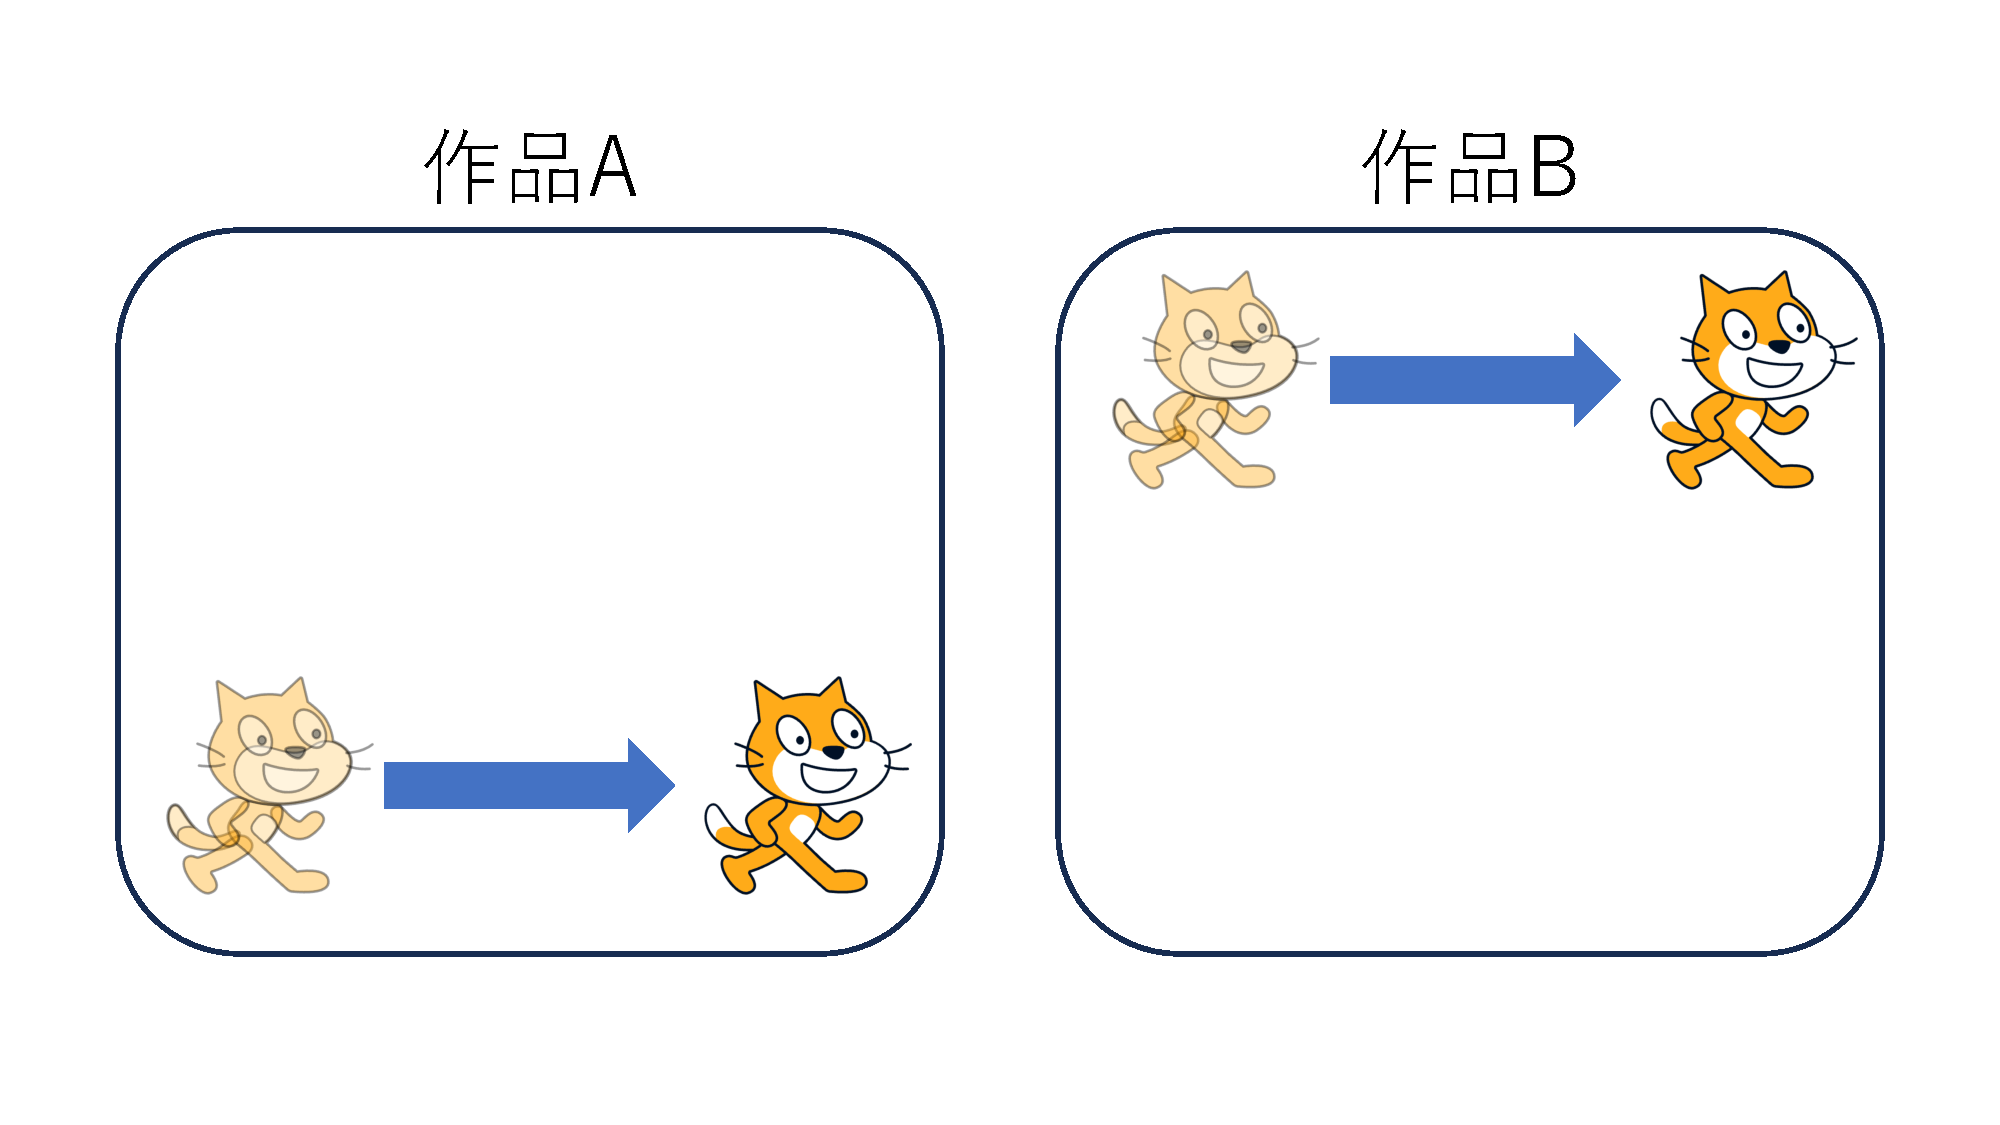
\includegraphics[width=1.0\linewidth]{Okamoto_fig/coordinate.pdf}
	\caption{座標が離れていて軌道が類似している作品例}
	\label{fig:coordinate}
\end{figure}

また,座標変化同士の距離は動的時間伸縮法(DTW: Dynamic time warping)を用いて算出する.DTWは2つの時系列データの距離を動的計画法に基づいて算出する手法である.DTWでは,2つの時系列データの各点の距離を総当たりで全て求め,2つの時系列データの累積距離が最短となる経路であるDTW距離を算出する.図\ref{fig:dtw}は,DTWの概念を示した図であるが,DTWでは,距離を算出する2つの時系列データS=$s_{1}$,$s_{2}$,$s_{3}$,…$s_{15}$, T=$t_{1}$,$t_{2}$,$t_{3}$,…$t_{10}$をそれぞれ縦軸,横軸に並べ,各マス(i,j)における要素$s_{i}$と$s_{j}$間の距離を算出する.図\ref{fig:dtw}中では,マスの色が薄いほど距離が近く,色が濃いほど距離が遠いことを指す.時系列データSとTの各要素の累積距離が最も短くなる経路を探し出し,その累積距離を2つの時系列データのDTW距離として算出する.DTW距離の値が小さいほど,動作軌跡の類似度は大きいと言える.
\begin{figure}[t]
	\centering
	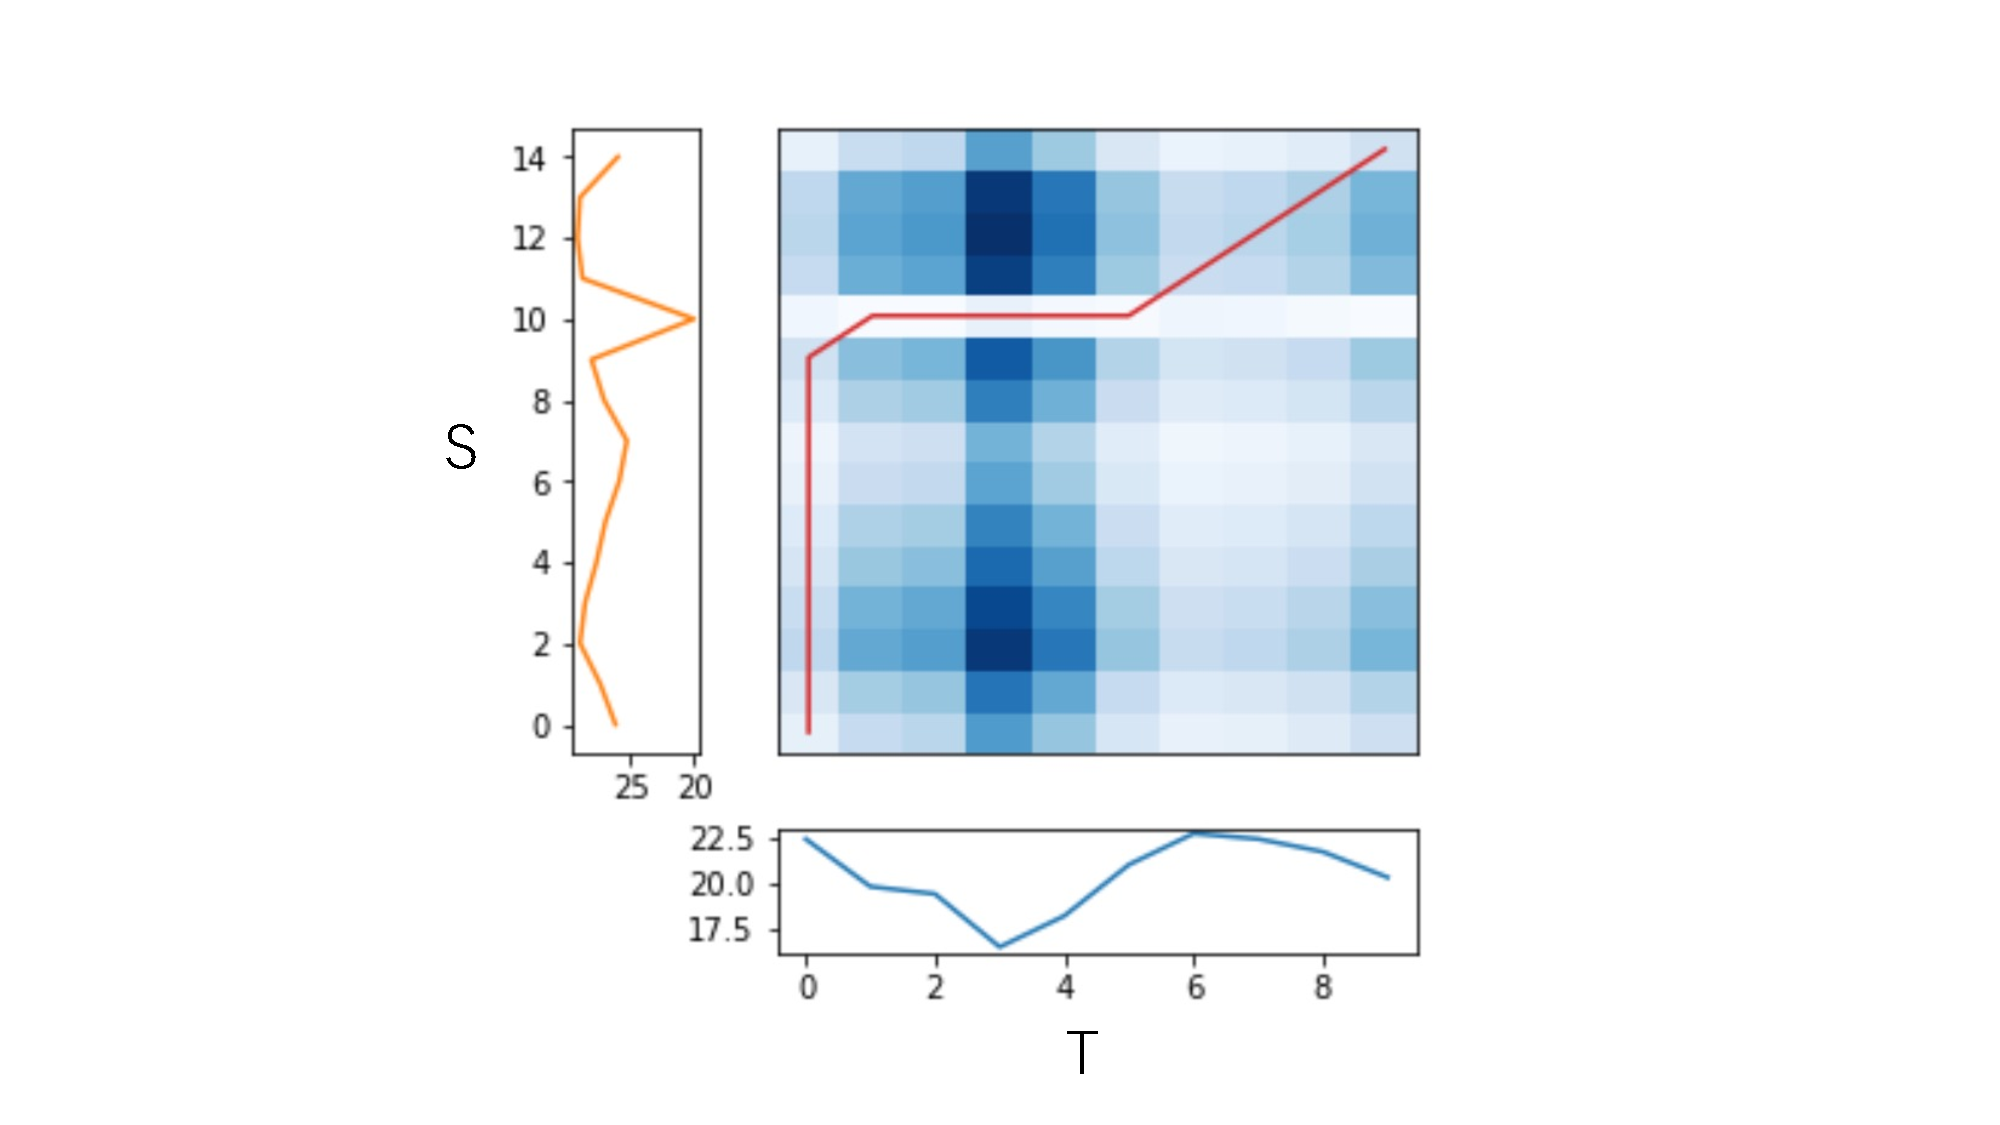
\includegraphics[width=1.0\linewidth]{Okamoto_fig/dtw.pdf}
	\caption{動的時間伸縮法(DTW)の概念図}
	\label{fig:dtw}
\end{figure}


\subsection{プログラムの類似度測定手法}\label{subsec:Similarity program measurement}

2.3節で述べた通り,テキストによるプログラム類似度の測定手法は多数提案されている.本研究では,Scratchで作成されるプログラムから抽象構文木を生成し,抽象構文木間の編集距離を用いてプログラム類似度を算出する.

\subsubsection{Scratchプログラムから抽象構文木への変換}

抽象構文木は,プログラムから言語の意味に関係のない情報を取り除き,意味に関係のある情報のみを取り出し,抽象化した木構造のデータである.

本研究では,Scratchが公開しているAPIを用いて作品情報を含むJSONファイルを入力として,スクリプトの情報を抽象構文木に変換する.
Scratchプログラムを抽象構文木に変換したときのイメージを図\ref{fig:abst}に示す.図\ref{fig:abst}の(1)に示すScratchプログラムを抽象構文木に変換すると,(2)となる.本研究で扱う抽象構文木では,(2)のようにブロック名をノードのラベルとし,1つのスクリプトにおけるすべてのブロックのつながりを示す.スクリプトは(2)に示したような「SCRIPT」を木の頂点とし,スクリプトの実行順序に従ってブロック名を左から1つの階層にノードラベルとして連ねる.制御ブロックをはじめとした,ブロックを内包する入れ子構造のブロックは,(2)に示した「gotoxy」,「turn」のように階層を1つ深くして表現する.また,本研究ではプログラム構造のみに着目して類似度を算出するため,制御ブロックが含む引数やその他の演算子等は考慮しない.
\begin{figure}[t]
	\centering
	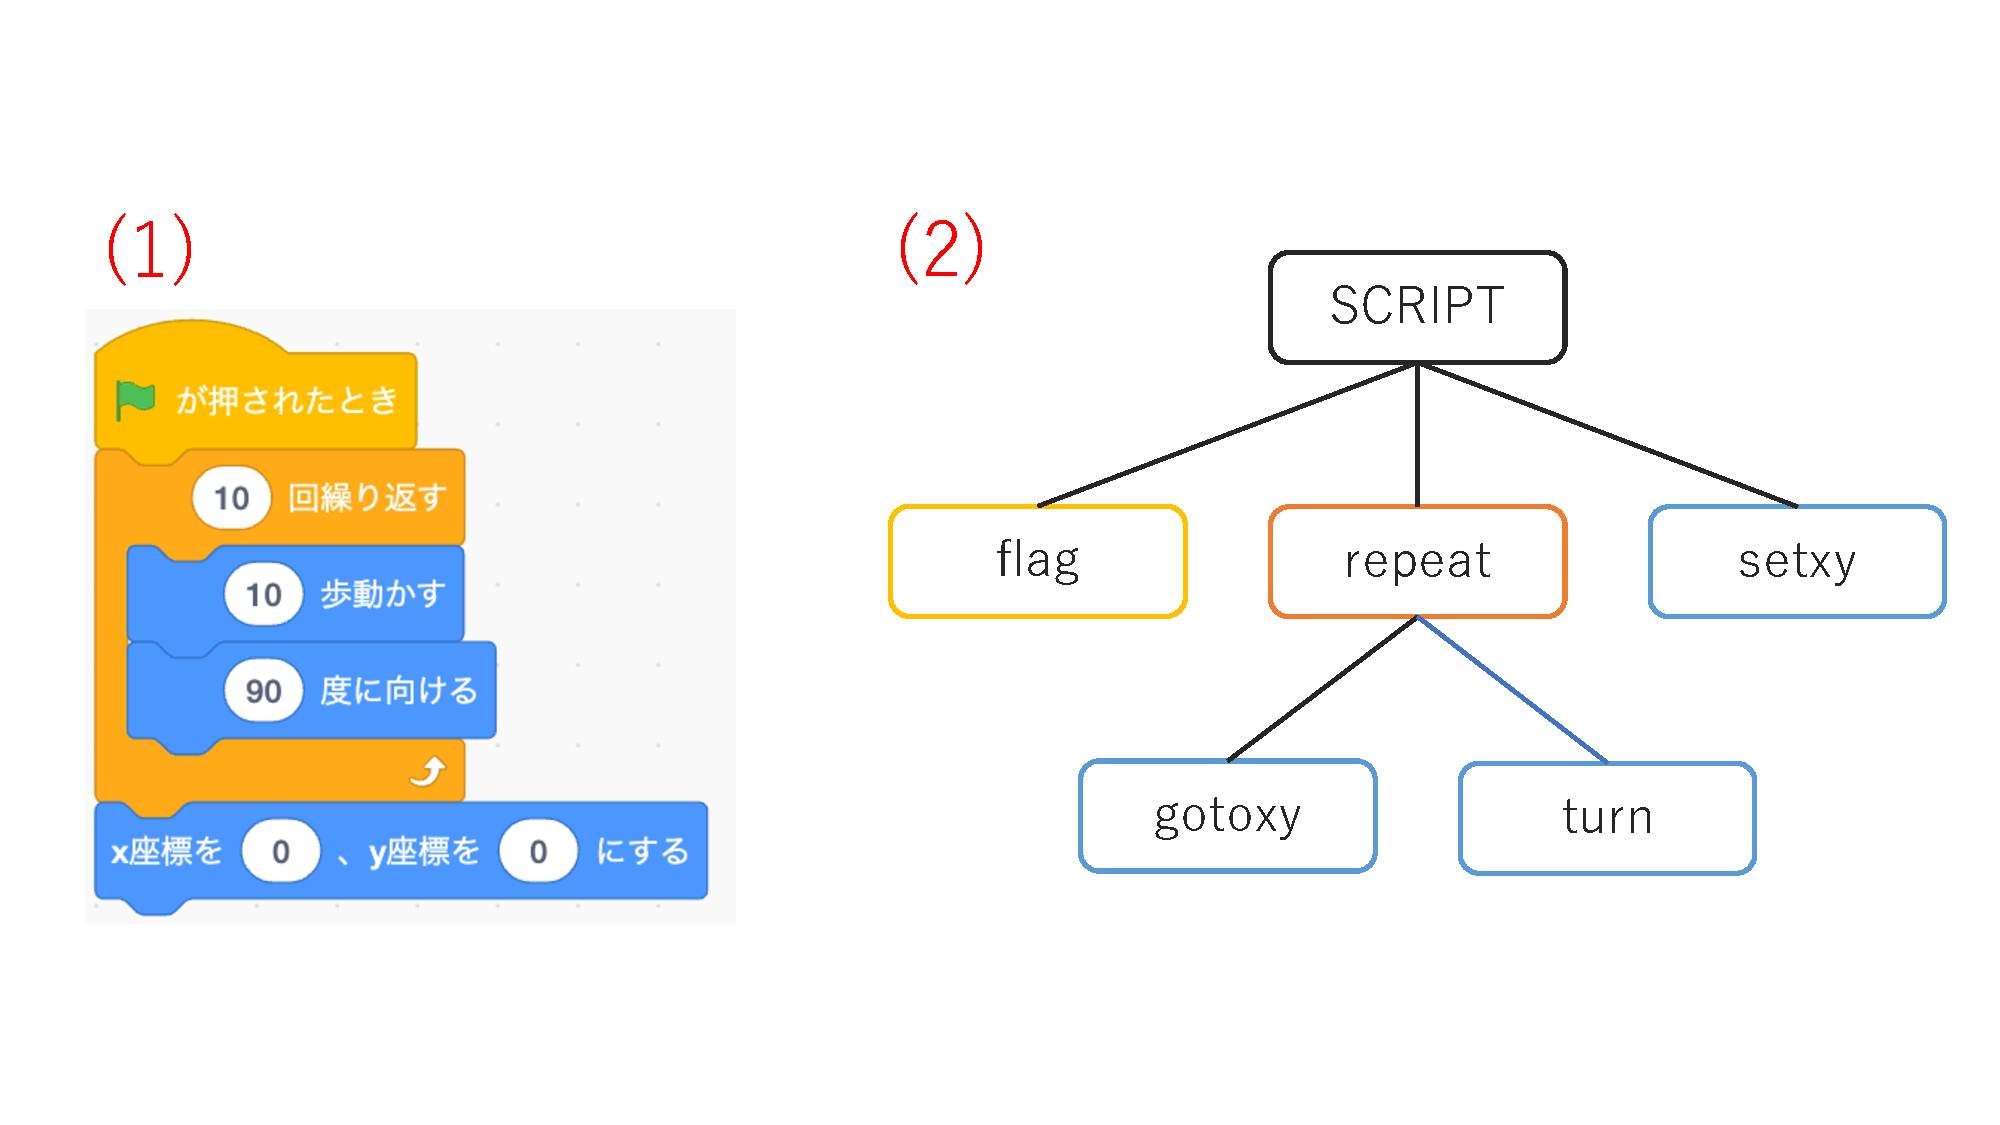
\includegraphics[width=1.0\linewidth]{Okamoto_fig/abst.pdf}
	\caption{Scratchプログラムから抽象構文木化}
	\label{fig:abst}
\end{figure}
%参考になりそう.https://sdl.ist.osaka-u.ac.jp/pman/pman3.cgi?DOWNLOAD=569

\subsubsection{編集距離によるプログラム類似度の算出}
異なる作品のスクリプトから変換した抽象構文木に基づき,抽象構文木間の編集距離を算出する.抽象構文木における編集距離とは,片方の抽象構文木をもう片方の抽象構文木と等しくするために行う最小の編集回数である.編集の定義は,ノードの挿入,ノードの削除,ノードラベルの置換の3種類であり,編集回数とはそれぞれを行った回数の合計数のことである.また,編集距離はブロックの長さに大きく影響を受けるため,算出した編集距離をブロック長が長い方の値で割り,最小値0,最大値1に正規化した値を編集距離とする.編集距離が小さいほど,プログラムの類似度は大きい.

%%%%%%%%%%%%%%%%%%%%%%
\section{動作軌跡類似度とプログラム類似度の関係性分析}\label{sec:Analyze related work}
%%%%%%%%%%%%%%%%%%%%%%

\subsection{データセット}
Scratchは,2019年のバージョン3.0のリリースにおいて,大幅なブロックの追加や仕様の変更が行われている.本研究では,共通の学習環境で制作された作品を比較するために,バージョン3.0がリリースされた2019年1月3日以降に制作された作品を対象とする.また,動作軌跡の計算を複雑化せず,ある程度のプログラム規模を持たせるため,以下の条件を満たす作品4000件を対象とした.
\begin{itemize}
    \item 並列に同じ種類のイベントブロックが存在しない
    \item 独自に定義するブロック,メッセージブロックが存在しない
    \item ブロック数が5つ以上
\end{itemize}
\subsection{アプローチ}\label{subsec:approach}
データセットとして収集した4000件の作品間の動作軌跡類似度,プログラム類似度を総当たりで測定し,作品対をプログラムが類似するか否か,スプライト動作軌跡が類似するか否かの4種類に分類する.また,プログラムと動作軌跡がそれぞれ類似しているかどうかは,先行研究で示された閾値に基づいて判断する.
\subsubsection{プログラム類似度の閾値}
先行研究では,編集距離を用いた類似スクリプトの紐付けを行った結果,閾値を0.50にしたときに最も分類の精度が高くなった.このことから,本研究では編集距離0.50をプログラムが類似する境界値とする.
\subsubsection{動作軌跡類似度の閾値}
先行研究では,DTWを用いた提案手法の精度を明らかにするために,著者が実装したScratch作品検索を用いて4種類の入力を行い,DTW距離の算出結果について分析を行った.定量分析では,距離を昇順に並べたある2点の傾きから距離が収束する値を求めることで,類似しない動作が抽出されるおおよその距離を明らかにした.定性分析では,定量分析で明らかにした距離以下の動作を提示し,動作の類似性を評価するアンケートを実施することで,類似動作を抽出可能な距離を4種類の入力それぞれについて明らかにした.本研究では,先行研究で示された4種類の入力と類似する動作を抽出可能な距離4つのうち,最もDTW距離の小さい2.2を動作軌跡が類似する境界値とする.
\subsection{結果}

図\ref{fig:out-nolimit}は,横軸に編集距離、縦軸にDTW距離を示し,それぞれの軸を対数表示した散布図である.
図中の1点は1つの作品対であることを表す.また,\ref{subsec:approach}で示した境界値を図中の線で示しており,この境界線に基づいて作品を4種類に分類した.

\begin{figure}[t]
	\centering
	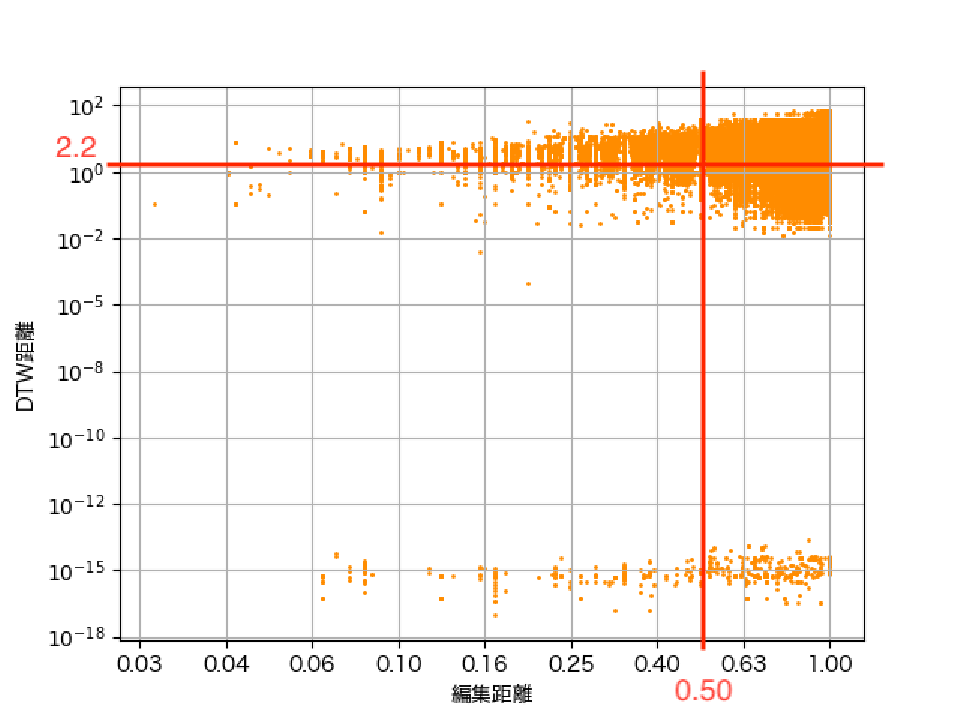
\includegraphics[width=1.0\linewidth]{Okamoto_fig/out-all-nolimit.pdf}
	\caption{DTW距離と編集距離の関係性を示した散布図}
	\label{fig:out-nolimit}
\end{figure}

\subsubsection{分析1:分類別の統計量}
表1は4つに分類された作品対の数を示した

\begin{table*}[ht]
    \centering
    \caption{分類別作品対数の比較}
    \begin{tabular}{|c|c|c|}
        \hline
        & プログラムが類似 & プログラムが類似しない \\
        \hline
        動作軌跡が類似 & \multicolumn{1}{c|}{98408} & \multicolumn{1}{c|}{2162523} \\
        \hline
        動作軌跡が類似しない & \multicolumn{1}{c|}{41877} & \multicolumn{1}{c|}{5293007} \\
        \hline
    \end{tabular}
    \captionsetup{skip=5pt}
    \label{table:programs-classification}
\end{table*}

\begin{table*}[ht]
    \centering
    \caption{分類別作品数の比較}
    \begin{tabular}{|c|c|c|}
        \hline
        & プログラムが類似 & プログラムが類似しない \\
        \hline
        動作軌跡が類似 & \multicolumn{1}{c|}{2842} & \multicolumn{1}{c|}{3603} \\
        \hline
        動作軌跡が類似しない & \multicolumn{1}{c|}{3017} & \multicolumn{1}{c|}{3889} \\
        \hline
    \end{tabular}
    \captionsetup{skip=5pt}
    \label{table:program-classification}
\end{table*}

\begin{table*}[ht]
    \centering
    \caption{分類別ブロック長平均値の比較}
    \begin{tabular}{|c|c|c|}
        \hline
        & プログラムが類似 & プログラムが類似しない \\
        \hline
        動作軌跡が類似 & \multicolumn{1}{c|}{15.5} & \multicolumn{1}{c|}{16.7} \\
        \hline
        動作軌跡が類似しない & \multicolumn{1}{c|}{15.4} & \multicolumn{1}{c|}{18.0} \\
        \hline
    \end{tabular}
    \captionsetup{skip=5pt}
    \label{table:program-length}
\end{table*}

\subsubsection{分析2:分類別のDTW距離の分布}
\begin{figure}[t]
	\centering
	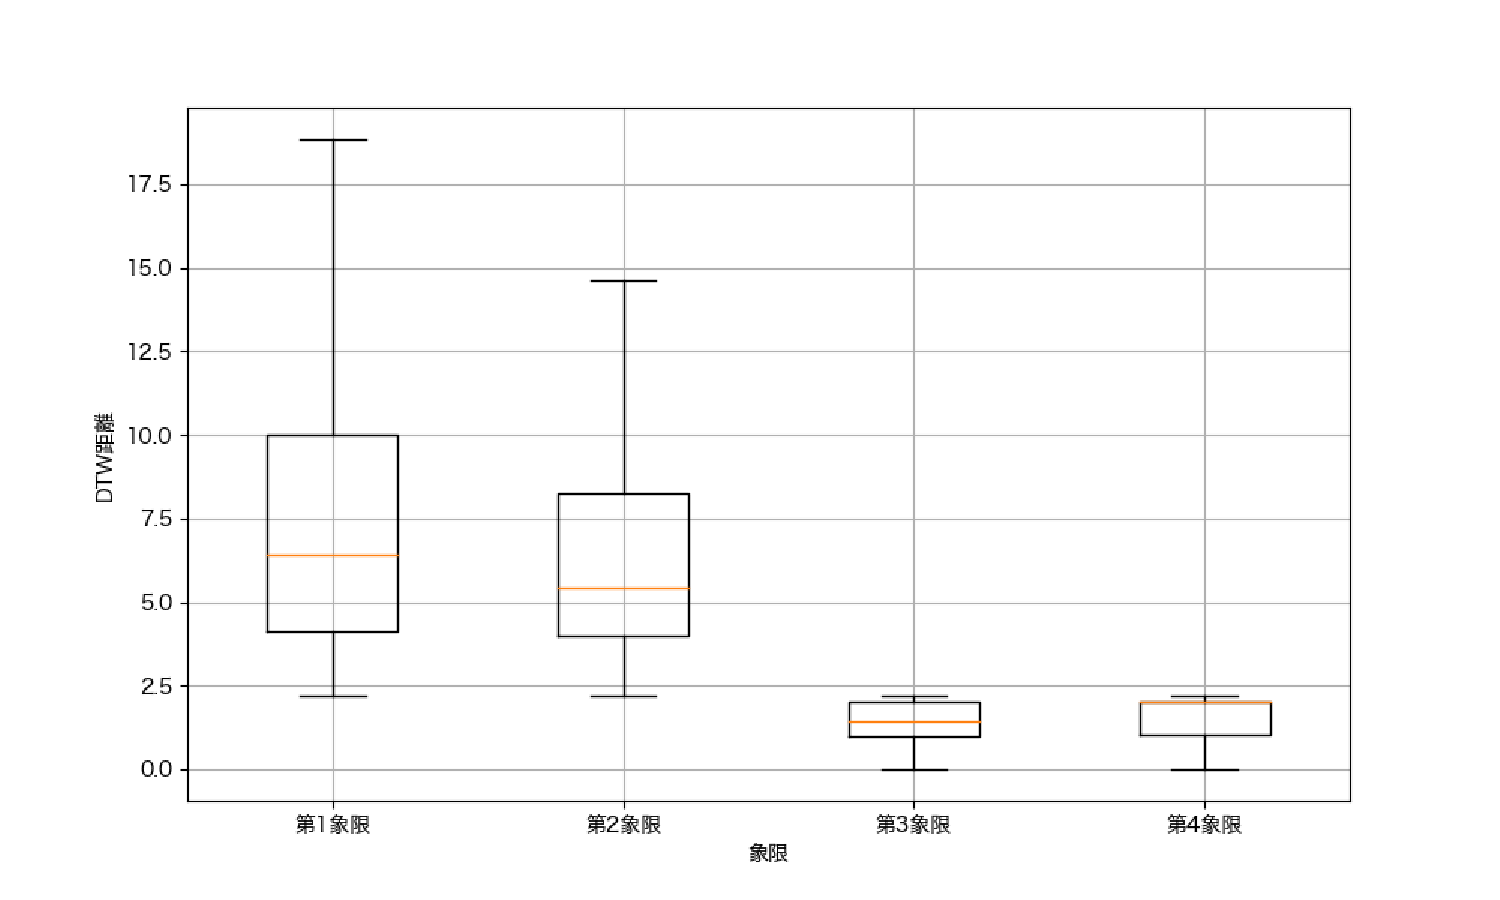
\includegraphics[width=1.0\linewidth]{Okamoto_fig/DTW-out.pdf}
	\caption{分類別にDTW距離の分布を示した箱ひげ図}
	\label{fig:dtw-boxplot}
\end{figure}

図\ref{fig:dtw-boxplot}は,4種類に分類した作品群毎にDTW距離の分布を示した箱ひげ図である.

\subsubsection{分析3:分類別の編集距離の分布}
\begin{figure}[t]
	\centering
	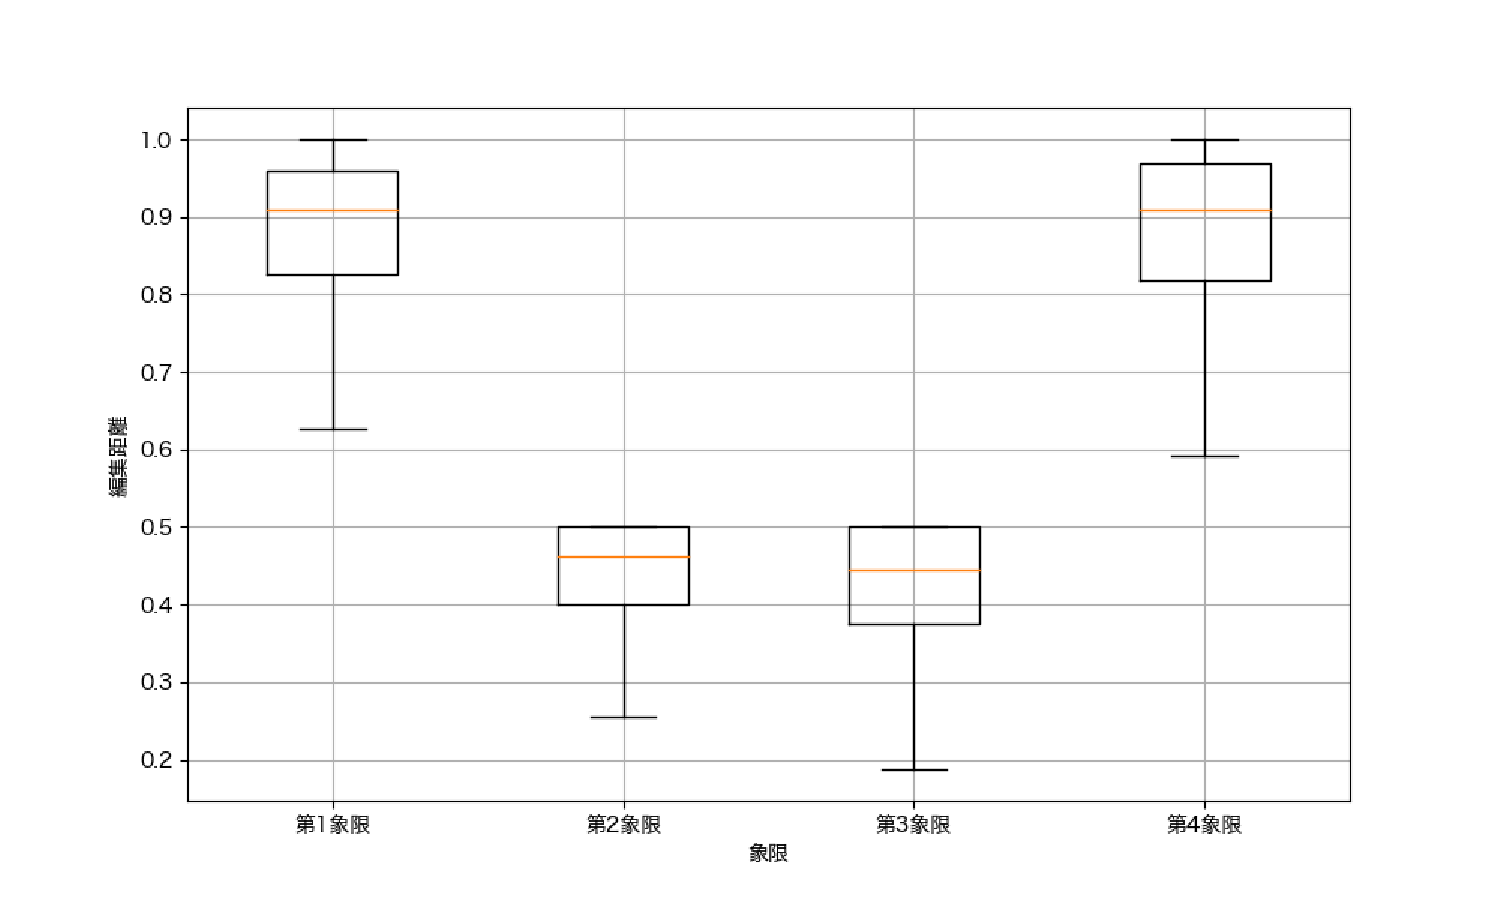
\includegraphics[width=1.0\linewidth]{Okamoto_fig/distance-out.pdf}
	\caption{分類別に編集距離の分布を示した箱ひげ図}
	\label{fig:distance-boxplot}
\end{figure}

% プログラムも動作軌跡も類似しない作品対
\begin{figure}[t]
	\centering
	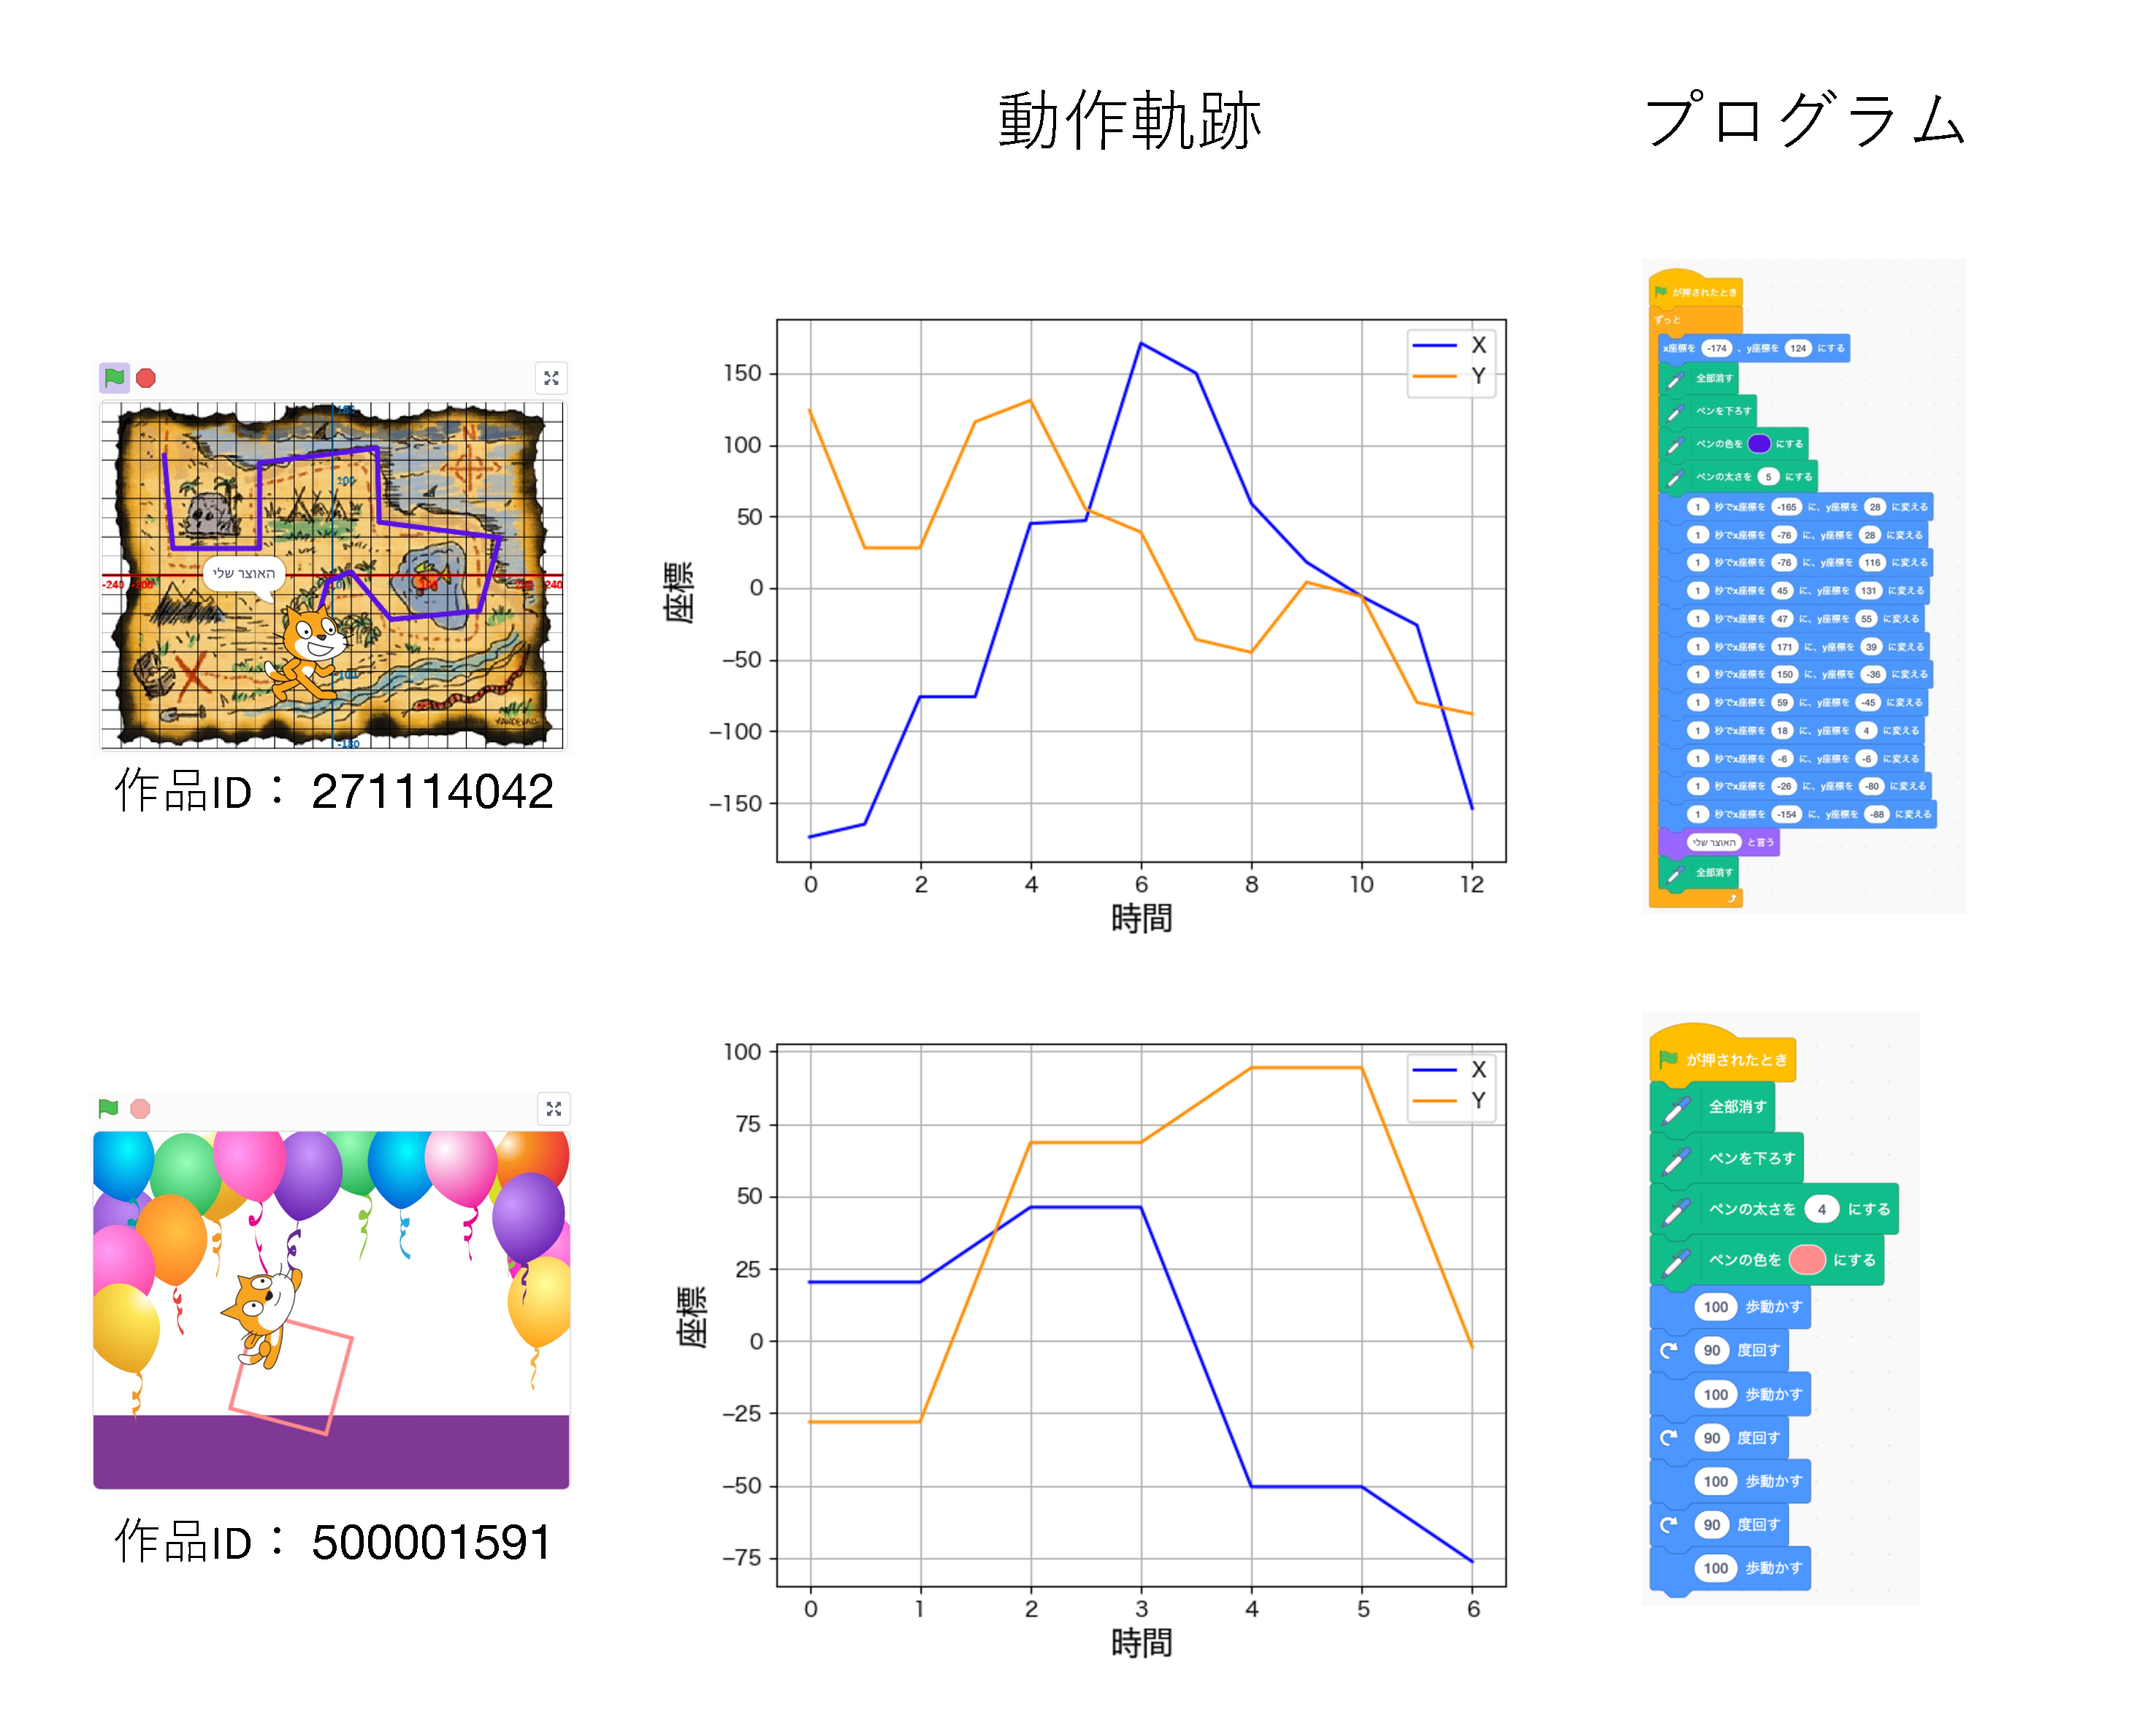
\includegraphics[width=1.0\linewidth]{Okamoto_fig/quadrant-1.pdf}
	\caption{DTW距離が7.92,編集距離が0.81の作品対}
	\label{fig:distance-boxplot}
\end{figure}

% プログラムは類似するが,動作軌跡は類似しない作品対
\begin{figure}[t]
	\centering
	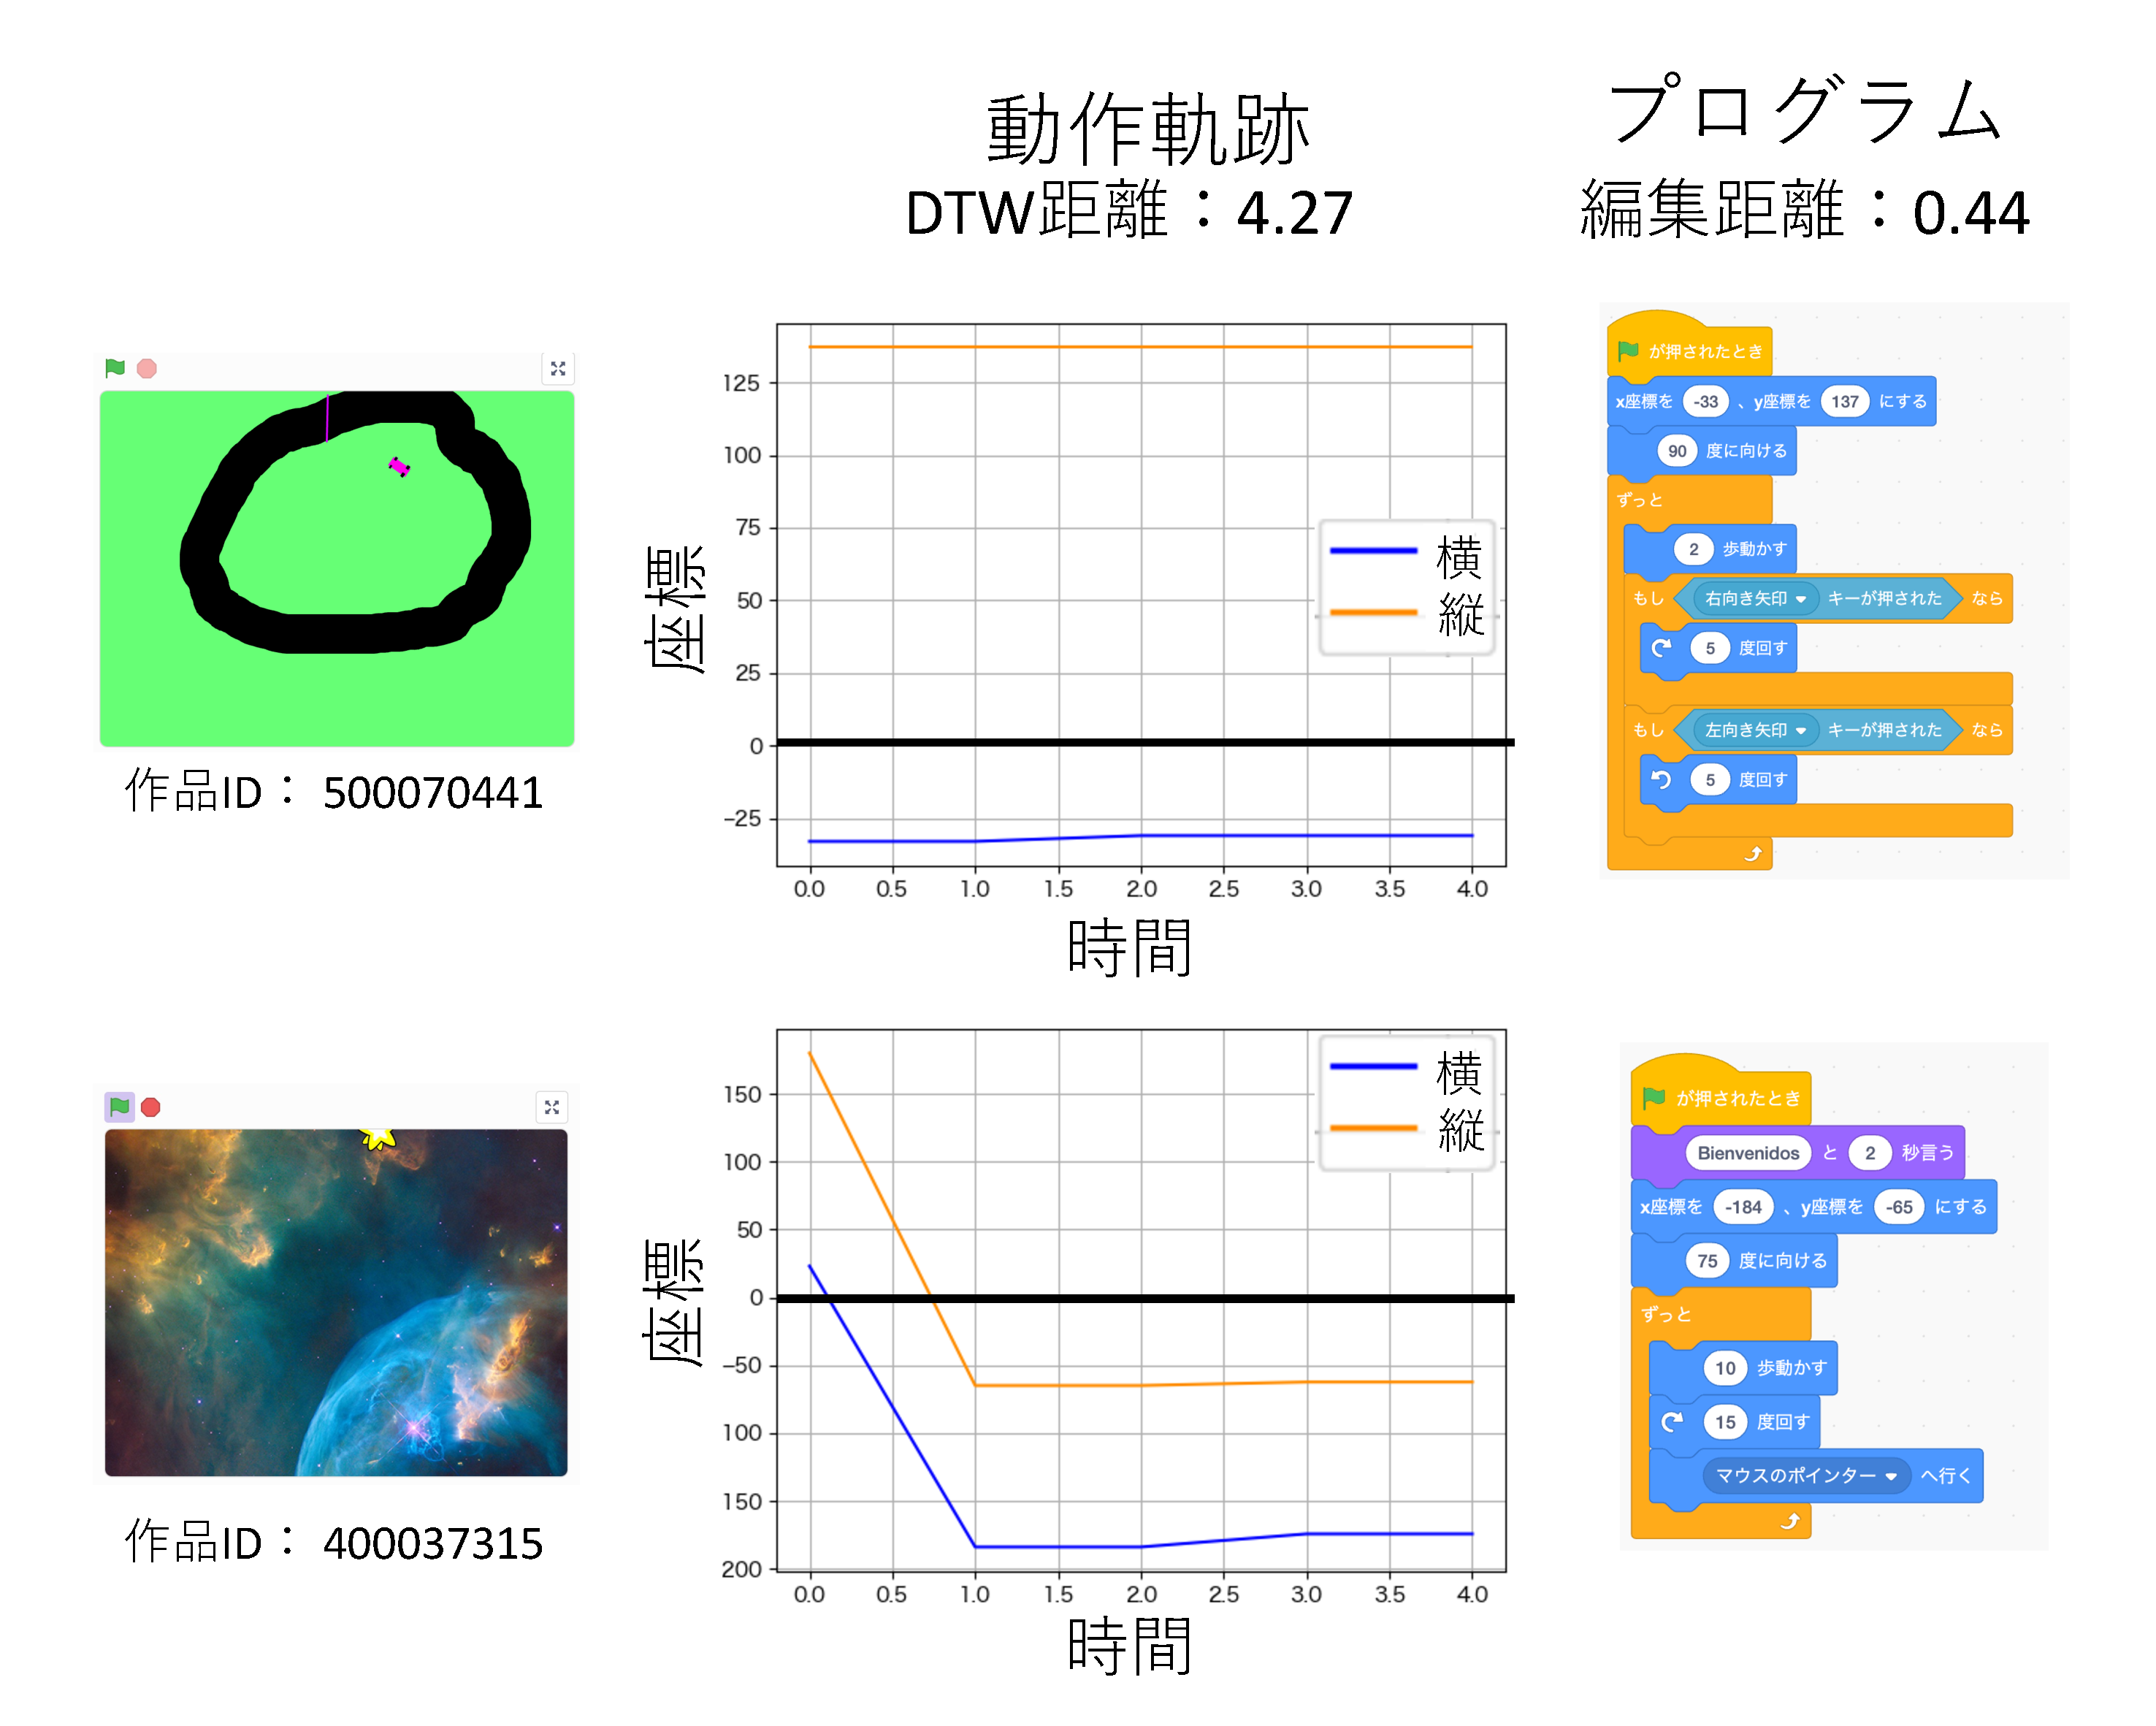
\includegraphics[width=1.0\linewidth]{Okamoto_fig/quadrant-2.pdf}
	\caption{DTW距離が4.27,編集距離が0.44の作品対}
	\label{fig:distance-boxplot}
\end{figure}

% プログラムも動作軌跡も類似する作品対
\begin{figure}[t]
	\centering
	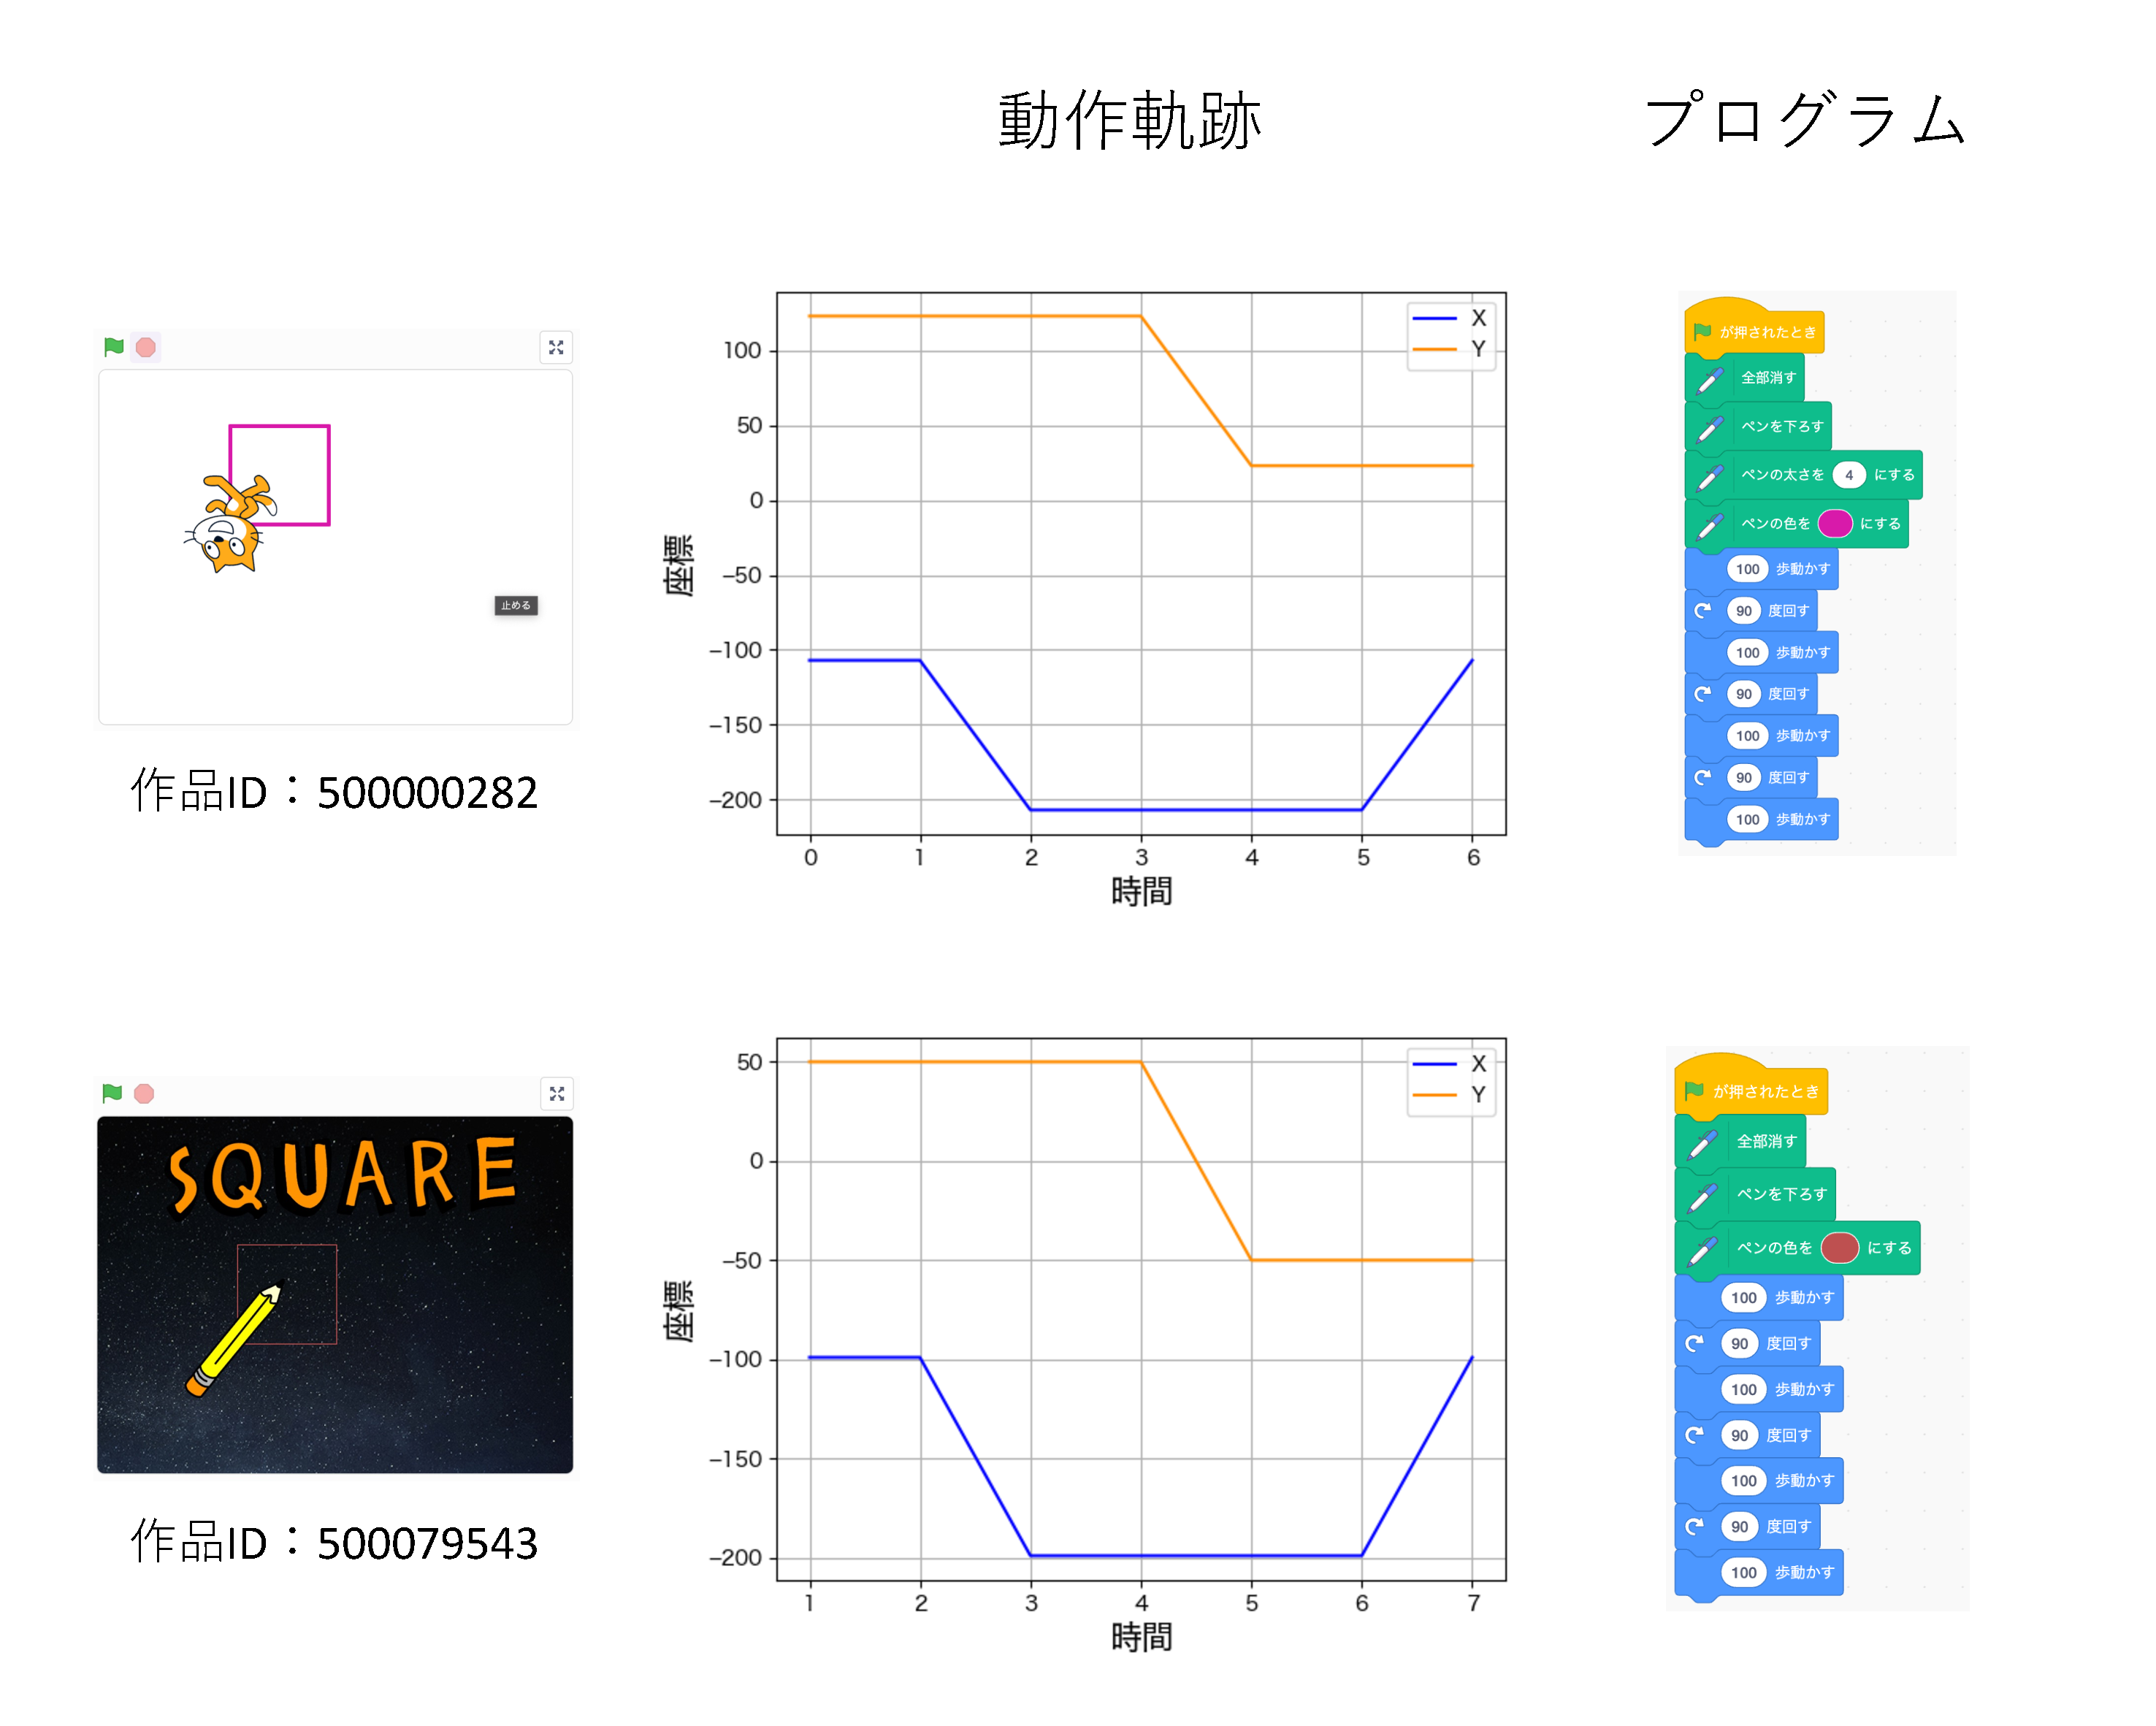
\includegraphics[width=1.0\linewidth]{Okamoto_fig/quadrant-3.pdf}
	\caption{DTW距離が1.003e-15,編集距離が0.08の作品対}
	\label{fig:distance-boxplot}
\end{figure}

% 動作軌跡は類似するが,プログラムは類似しない作品対
\begin{figure}[t]
	\centering
	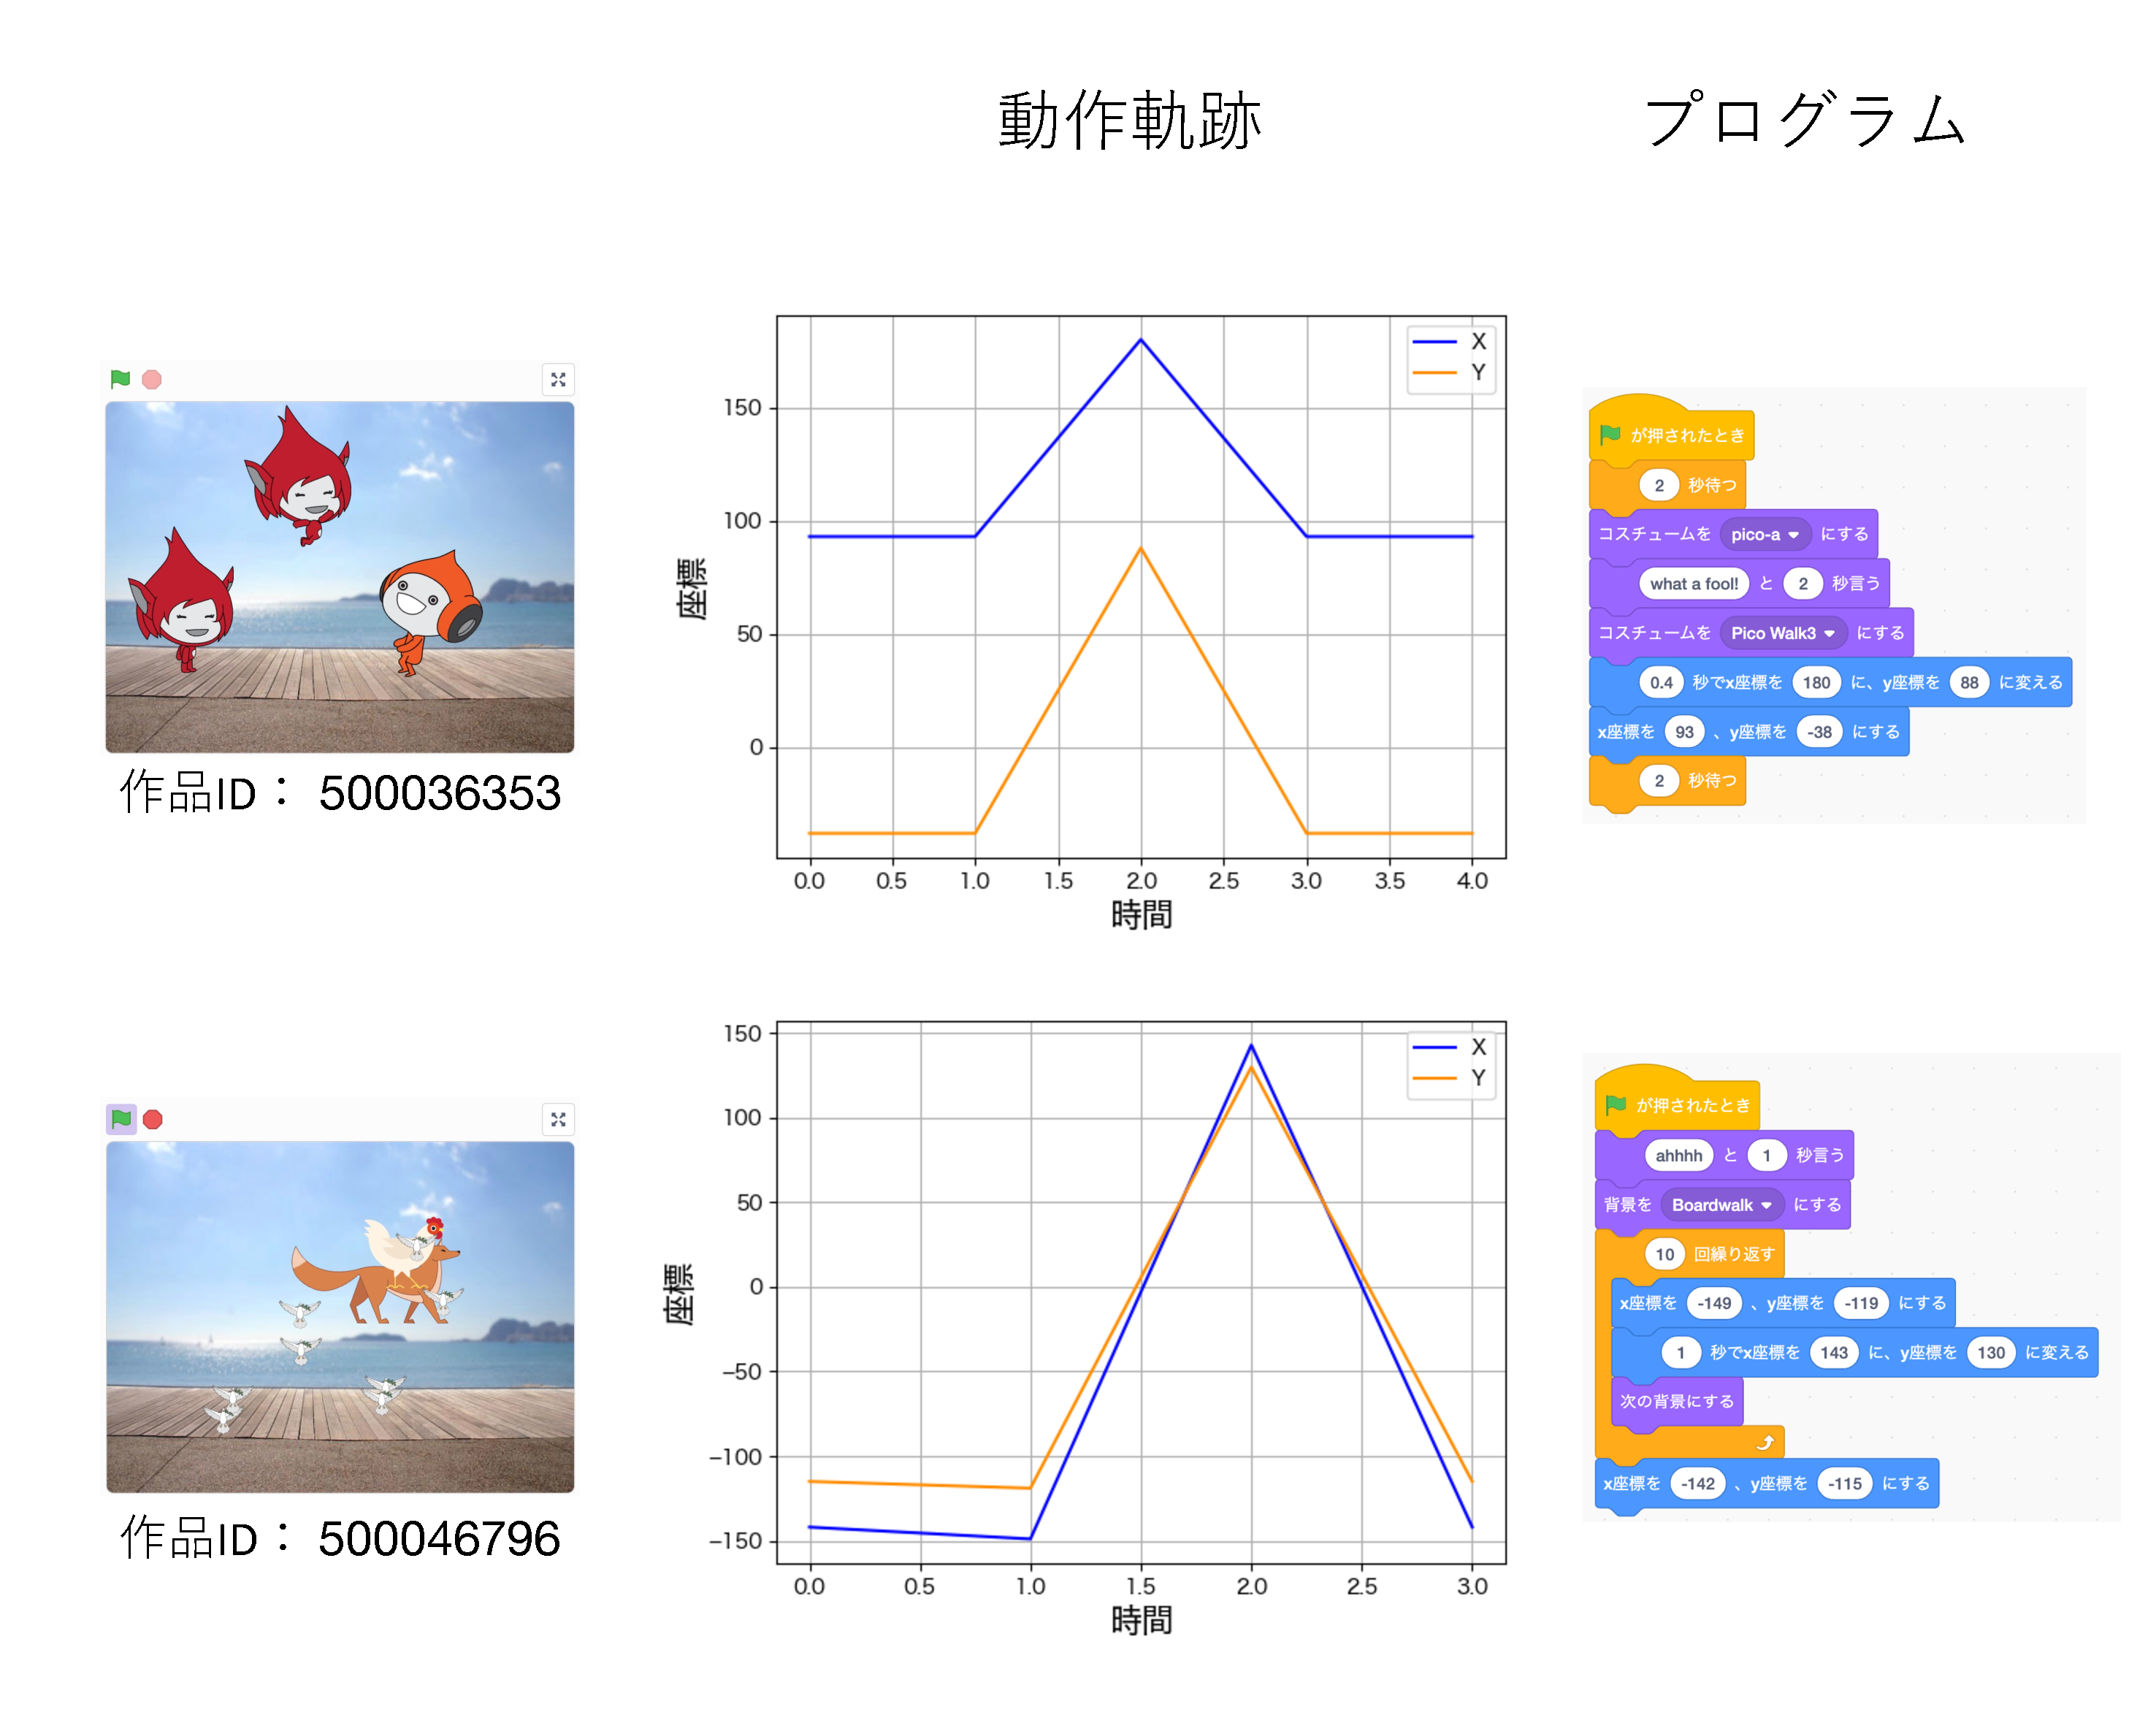
\includegraphics[width=1.0\linewidth]{Okamoto_fig/quadrant-4.pdf}
	\caption{DTW距離が0.087,編集距離が0.88の作品対}
	\label{fig:distance-boxplot}
\end{figure}

\subsubsection{考察}



\section{おわりに}


%\begin{adjustvboxheight} % needed only when Appendix follows
\bibliographystyle{junsrt}
\bibliography{okamoto}

%\end{adjustvboxheight} % needed only when Appendix follows

% 以下はbibtexを使用しない場合の例です.
% 332行目と333行目をコメントアウトしてから使用してください.
% なお,この例では年数順に文献が並んでいるので適切な並び順ではありません.
%\begin{adjustvboxheight} % needed only when Appendix follows
%\begin{thebibliography}{9}
%\bibitem{fose2021} 名倉 正剛,関澤 俊弦 編:ソフトウェア工学の基礎28,日本ソフトウェア科学会{\em FOSE2021}, 近代科学社, 2021.
%\bibitem{fose2022} 角田 雅照,まつ本 真佑 編:ソフトウェア工学の基礎29,日本ソフトウェア科学会{\em FOSE2022}, 近代科学社, 2022.
%\bibitem{fose2023} 吉田 則裕,槇原 絵里奈 編:ソフトウェア工学の基礎30,日本ソフトウェア科学会{\em FOSE2023}, 近代科学社, 2023. (to appear)
%\end{thebibliography}
%\end{adjustvboxheight} % needed only when Appendix follows

%以下は付録の例です.必要ならコメントアウトして使用してください.
%なお,その際には参考文献の前後にある adjustvboxheight 環境のコメントアウトを解除してください.
%\appendix
%\section{付録A} 
%これは付録の例です.

\end{document}


